\section{Method for generating permeability fields }

Due to incomplete data about rock properties that show variability at multiple length scales, input parameters such as the permeability field, $\perm(\vx,\ale)$, are treated as random space functions with statistics inferred from geostatistical models (here $\vx =\left( x_{1},x_{2},x_{3}  \right)^{\! ^{\mathsf{T}}}\in \mathbb{R}^{3}$ and $\ale$ is a random element in the probability space).
In line with \cite{dagan89} and \cite{gelhar93} the permeability field is modeled as a log-normally distributed random space function
%
\begin{equation}
  \perm\fxw = \exp\left[\Y\fxw\right],
\label{field}
\end{equation}
%
\noindent where $\Y\fxw \sim \normal{\me{\Y}}{\cov{\Y}}$ is a Gaussian random field
characterized by its mean $\me{\Y} = \med{\Y}$ and two-point covariance function

\begin{equation}
 \covv{\Y} = \covar{\Y\fx}{\Y\fy} = \mathsf{E}\big[ \left( \Y\fx - \med{\Y\fx}  \right) \left( \Y\fy - \med{\Y\fy}  \right) \big].
 \label{covg}
\end{equation}
%

The Gaussian field $\Y$ can be represented as a series expansion involving a complete set of deterministic functions with correspondent random coefficients using the \KL\ (\kl)
expansion, proposed independently by \cite{karhunen46} and \cite{loeve55}. 
It is based on the eigen-decomposition of the covariance function.
Depending on how fast the eigenvalues decay one may be able to  retain only a small number of terms in a truncated expansion and, consequently, this procedure may reduce the search to a smaller parameter space.
In uncertainty quantification methods for porous media flows, the \kl\ expansion has been widely used to reduce the number of parameters used to represent the permeability field
\citep{efendiev05,efendiev2006,das10,mondal10,ginting11,ginting12}.
Another advantage of \kl\ expansion lies on the fact that it provides orthogonal deterministic basis functions and uncorrelated random coefficients, allowing for the optimal encapsulation of the information contained in the random process into a set of discrete uncorrelated random variables \citep{GhanemSpanos}. 
This remarkable feature can be used to simplify the Metropolis-Hastings \mcmc\
Algorithm in the sense of the search may be performed in the space of discrete uncorrelated
random variables ($\vtheta$), no longer in the space of permeabilities which have a more complex statistical structure.

%%%%%%%%%%%%%%%%%%%%%%%%%%%%%%%%%%%%%%%%%%%%%%%%%%%%%%%%%%%%%%%%%%%%%%%%%%%%%%%%%%%%%%%%%%%%%%%%%%%%%%%%%%%%%%%%%%%%%%%%%%%%%%%%%%%%
%%%%%%%%%%%%%%%%%%%%%%%%%%%%%%%%%%%%%%%%%%%%%%%%%%%%%%%%%%%%%%%%%%
Here we recall the basic facts about the \KL\ expansion. 
Consider a random field $\Y(\vx,\ale)$ defined on a probability space $(\Omega,\events,\probab)$ composed by the sample space, the ensemble of events and a probability measure, respectively, and indexed on a bounded domain $\D \in \mathbb{R}^{3}$.
The process $\Y$ can be expressed as 
%
\begin{equation}
  \Yxw = \med{\Y(\vx)} +\sum_{i=1}^{\infty}\sqrt{\avai} \avei(\vx)
\theta_{i}(\ale),
\label{kl}
\end{equation}
%
\noindent where $\avai$ and $\avei$ are the eigenvalues and eigenfunctions of the covariance function $\covv{\Y}$, respectively. 
By definition, $\covv{\Y}$ is bounded, symmetric and positive definite and has the following eigen-decomposition:
%
\begin{equation*}
  \covv{\Y} = \sum_{i=1}^{\infty} \avai\avei(\vx)\avei(\vy).
\label{klcov}
\end{equation*}
%

The eigenvalues and eigenfunctions of \eq{kl} are the solution of the homogeneous Fredholm integral equation of second kind given by
%
\begin{equation}
  \int_{\D} \covv{\Y} \ave(\vx) d\vx = \ava\ave(\vy).
\label{fred}
\end{equation}
%
\noindent The solution of \eq{fred} forms a complete set of a square-integrable
orthogonal eigenfunctions that satisfy the equation
%
\begin{equation*}
  \int_{\D} \avei(\vx) \avej(\vx)=\delta_{ij},
\label{ortho}
\end{equation*}
%
\noindent in which $\delta_{ij}$ is the Kronecker-delta function.
$\theta_{i}(\ale)$ is a set of independent random variables which
can be expressed as
%
\begin{equation*}
  \theta_{i}(\ale) = \displaystyle
\frac{1}{\sqrt{\avai}}\int_{\D}\flu{\Y}\avei(\vx) d\vx,
\end{equation*}
%
\noindent where $\flu{\Y}=\Y-\med{\Y}$ is the fluctuation.
For practical implementations of the \kl\ expansion the eigenvalues are arranged from the largest to smallest and the series is approximated by a finite number of terms, say the first $\mm$, giving
%
\begin{equation}
  \Y\fxw \approx \med{\Y(\vx)} +\sum_{i=1}^{\mm}\sqrt{\avai} \avei(\vx)
\theta_{i}(\ale).
\label{klM}
\end{equation}
%
The corresponding covariance function is given by 
%
\begin{equation*}
  \covv{\Ym} = \sum_{i=1}^{\mm} \avai\avei(\vx)\avei(\vy).
\label{klcovM}
\end{equation*}
%

The factors affecting the convergence of the \KL\ series are the ratio of the length of the process over correlation parameter, the form of the covariance function, and the solution method for the eigensolutions of the covariance function (see \cite{huang01}). 
Next we discuss the field conditioning using the \kl\ expansion.

%%%%%%%%%%%%%%%%%%%%%%%%%%%%%%%%%%%%%%%%%%%%%%%%%%%%%%%%%%%%%%%%%%%%%%%%%%%%%%%%%%%%%%%%%%%%%%%%%%%%
%%%%%%%%%%%%%%%%%%%%%%%%%%%%%%%%%%%%%%%%%%%%%%%%%%%%%%%%%%%%%%%%%%%%%%%%%%%%%%%%%%%%%%%%%%%%%%%%%%%%
%%%%%%%%%%%%%%%%%%%%%%%%%%%%%%%%%%%%%%%%%%%%%%%%%%%%%%%%%%%%%%%%%%%%%%%%%%%%%%%%%%%%%%%%%%%%%%%%%%%%
\subsection{Conditioning procedure}\label{sec:klcond}

From measurements obtained in samples, the permeability field is known at sparse locations and this information can be incorporated in the \apri\ distribution.

Suppose that the Gaussian field $\Y$ (as well as the permeability field $\perm$ of \eq{field}) is known at $\nc$ positions $\left\{ \pvx_{i}\right\}_{i=1}^{\nc}$, that is:
\begin{equation}
 \Y \left( \pvx_{i} \right) = \Y_{i},\quad i=1,\dots,\nc.
\end{equation}

To honor these measures in the field generation process with the \kl\ expansion we consider the projection of random vector $\vtheta = \left[\theta_{1}, \theta_{2},\dots  \right]^{\mathsf{T}}$ (\eq{kl}) onto an appropriate subspace as proposed by \cite{Ossiander2014}.
In their method the original $\vtheta$ is replaced by its projection $\proj{\vtheta}$ that has the same distribution as the original. 
Next, we briefly describe the method for the \kl\ expansion truncated at $\mm$ term.

Let $\mS\in\real^{\nc\times\nc}$ be the covariance matrix of the observed locations

\begin{equation}
 \mS_{k,j} \equiv \cov{\Y}\left( \pvx_{k}, \pvx_{j} \right) =
 \sum_{i=1}^{\mm} \avai\avei(\pvx_{k})\avei(\pvx_{j}),
 \quad k,j = 1,\dots,\nc.
\end{equation}

\noindent Next, define $\R^{\mm\times\nc}$ to be the matrix with the columns given by the eigenfunctions at the observed locations $\left\{ \pvx_{i}\right\}_{i=1}^{\nc}$, then

\begin{equation}
 \R \equiv \Big[ \avei(\pvx_{1}),\avei(\pvx_{2}),\dots,\avei(\pvx_{\nc}) \Big].
 \label{mR}
\end{equation}

\noindent By the last definition and making $\mava$ the diagonal matrix of eigenvalues $\avai$ ($i=1,\dots,\mm$), $\mS$ can be rewritten as

\begin{equation*}
 \mS = \R^{\mathsf{T}}\mava\R.
\end{equation*}

To compute the mean $\proj{\me{\theta}}$ and covariance $\covM{} = (m_{i,k})$ of the sequence of random variables $\left\{ \theta_{i} \right\}_{i=1}^{\mm}$ conditioned on $\pX = \left\{ \pvx_{i}\right\}_{i=1}^{\nc}$ an usual formula for conditional means and covariance of Gaussian variables is used \citep{tong1990multivariate}:

\begin{equation}
 \proj{\me{\theta,i}} = \mathsf{E}\left[ \theta_{i} | \pX \right] = \sqrt{\avai}\avei(\pvx) \mS^{-1} \left[ \Y(\pvx) - \med{\Y(\pvx)} \right]
\end{equation}

\noindent and

\begin{equation}
 \begin{array}{rcl}
  m_{i,j} &=& \covar{\theta_{i}}{\theta_{j}|\pX}\\
          &=& \delta_{i,j} - \sqrt{\avaj}\avej(\pvx) \mS^{-1} \avei(\pvx)\sqrt{\avai}.
 \end{array}
\label{mmatrix}
\end{equation}

\noindent Thus, the projection matrix is given by

\begin{equation}
 \covM{} = \boldsymbol{\mathsf{I}} - \mava^{1/2}\ \R\ \mS^{-1}\ \R^{\mathsf{T}} \ \mava^{1/2},
\end{equation}

\noindent where $\boldsymbol{\mathsf{I}}$ is the identity matrix.
Finally the vector $\vtheta$ conditioned on $\pX$ is given by

\begin{equation}
 \proj{\vtheta} = \proj{\me{\vtheta}} + \covM{} \vtheta.
\end{equation}

\noindent Here $\covM{}$ projects $\vtheta$ onto the subspace that gives the $\proj{\Y}$ process conditional variance 0 at the locations $\left\{ \pvx_{i}\right\}_{i=1}^{\nc}$.
The conditional representation $\proj{\Y}\fx$ of ${\Y\fx}$ reads as

\begin{equation}
  \proj{\Y}\fxw \approx \med{{\Y}(\vx)} +\sum_{i=1}^{\mm}\sqrt{\avai} \avei(\vx) \proj{\theta_{i}}(\ale),
  \quad \vx \in \D.
\label{klM}
\end{equation}

The matrix $\covM{}$ projects the $\mm$ dimensional vector $\vtheta$ onto the $\mm - \nc$ dimensional subspace.
Then, in order to have a sufficient number of degrees of freedom for the projection, we must have $\mm > \nc$

The number of terms used in the series can be chosen based on the energy represented by the sum of the eigenvalues. 
Then we define the relative energy for $n$ terms as

\begin{equation}
 \re{n} = \dfrac{\sum_{i=1}^{n}\avai}{\sum_{j=1}^{m\rightarrow\infty}\avaj}.
\end{equation}


%%%%%%%%%%%%%%%%%%%%%%%%%%%%%%%%%%%%%%%%%%%%%%%%%%%%%%%%%%%%%%%%%%
%%%%%%%%%%%%%%%%%%%%%%%%%%%%%%%%%%%%%%%%%%%%%%%%%%%%%%%%%%%%%%%%%%
\section{Numerical experiments}
%%%%%%%%%%%%%%%%%%%%%%%%%%%%%%%%%%%%%%%%%%%%%%%%%%%%%%%%%%%%%%%%%%

To test the implemented code, numerical experiments were performed, in which sets of 5000 fields (conditioned and unconditioned). 
Different covariance functions ($\covv{\Y}$), correlation lengths ($\cc$) and number of expansion terms ($\mm$) were used in the tests.
After obtaining the fields, the mean and covariance of the sets were computed and compared with the expected values.

In all cases, three-dimensional fields were generated with dimensions: $1.0 \times 0.6 \times 0.4$ and mesh $25 \times 15 \times 10$.
%%%%%%%%%%%%%%%%%%%%%%%%%%%%%%%%%%%%%%%%%%%%%%%%%%%%%%%%%%%%%%%%%%
\subsection{Squared Exponential Covariance}
%%%%%%%%%%%%%%%%%%%%%%%%%%%%%%%%%%%%%%%%%%%%%%%%%%%%%%%%%%%%%%%%%%
The two-point squared exponentially decaying covariance function
is given by
\begin{equation}
 \covv{\Y} = \vari{\Y}\exp\left(-\dfrac{\norma{x_1 - y_1}^2}{\cc_{1}^{2}}-\dfrac{\norma{x_2 - y_2}^2}{\cc_{2}^{2}}-\dfrac{\norma{x_3 - y_3}^2}{\cc_{3}^{2}}  \right),
 \label{eq-squarecov}
\end{equation}

\noindent with $\vari{\Y}$ denoting the variance and $\cc_{i}>0,\ i=1,2,3$ the correlation length in each cartesian direction.
More specifically, in this study, $\ell_{1}=0.25$, $\ell_{2}=0.20$ and $\ell_{3}=0.15$.

%%%%%%%%%%%%%%%%%%%%%%%%%%%%%%%%%%%%%%%%%%%%%%%%%%%%%%%%%%%%%%%%%%
\subsubsection{Unconditioned}

Two realizations of the fields are displayed in \fig{fig-uncondFields}.

\begin{figure}[H]
 \centering
 \subfigure[]{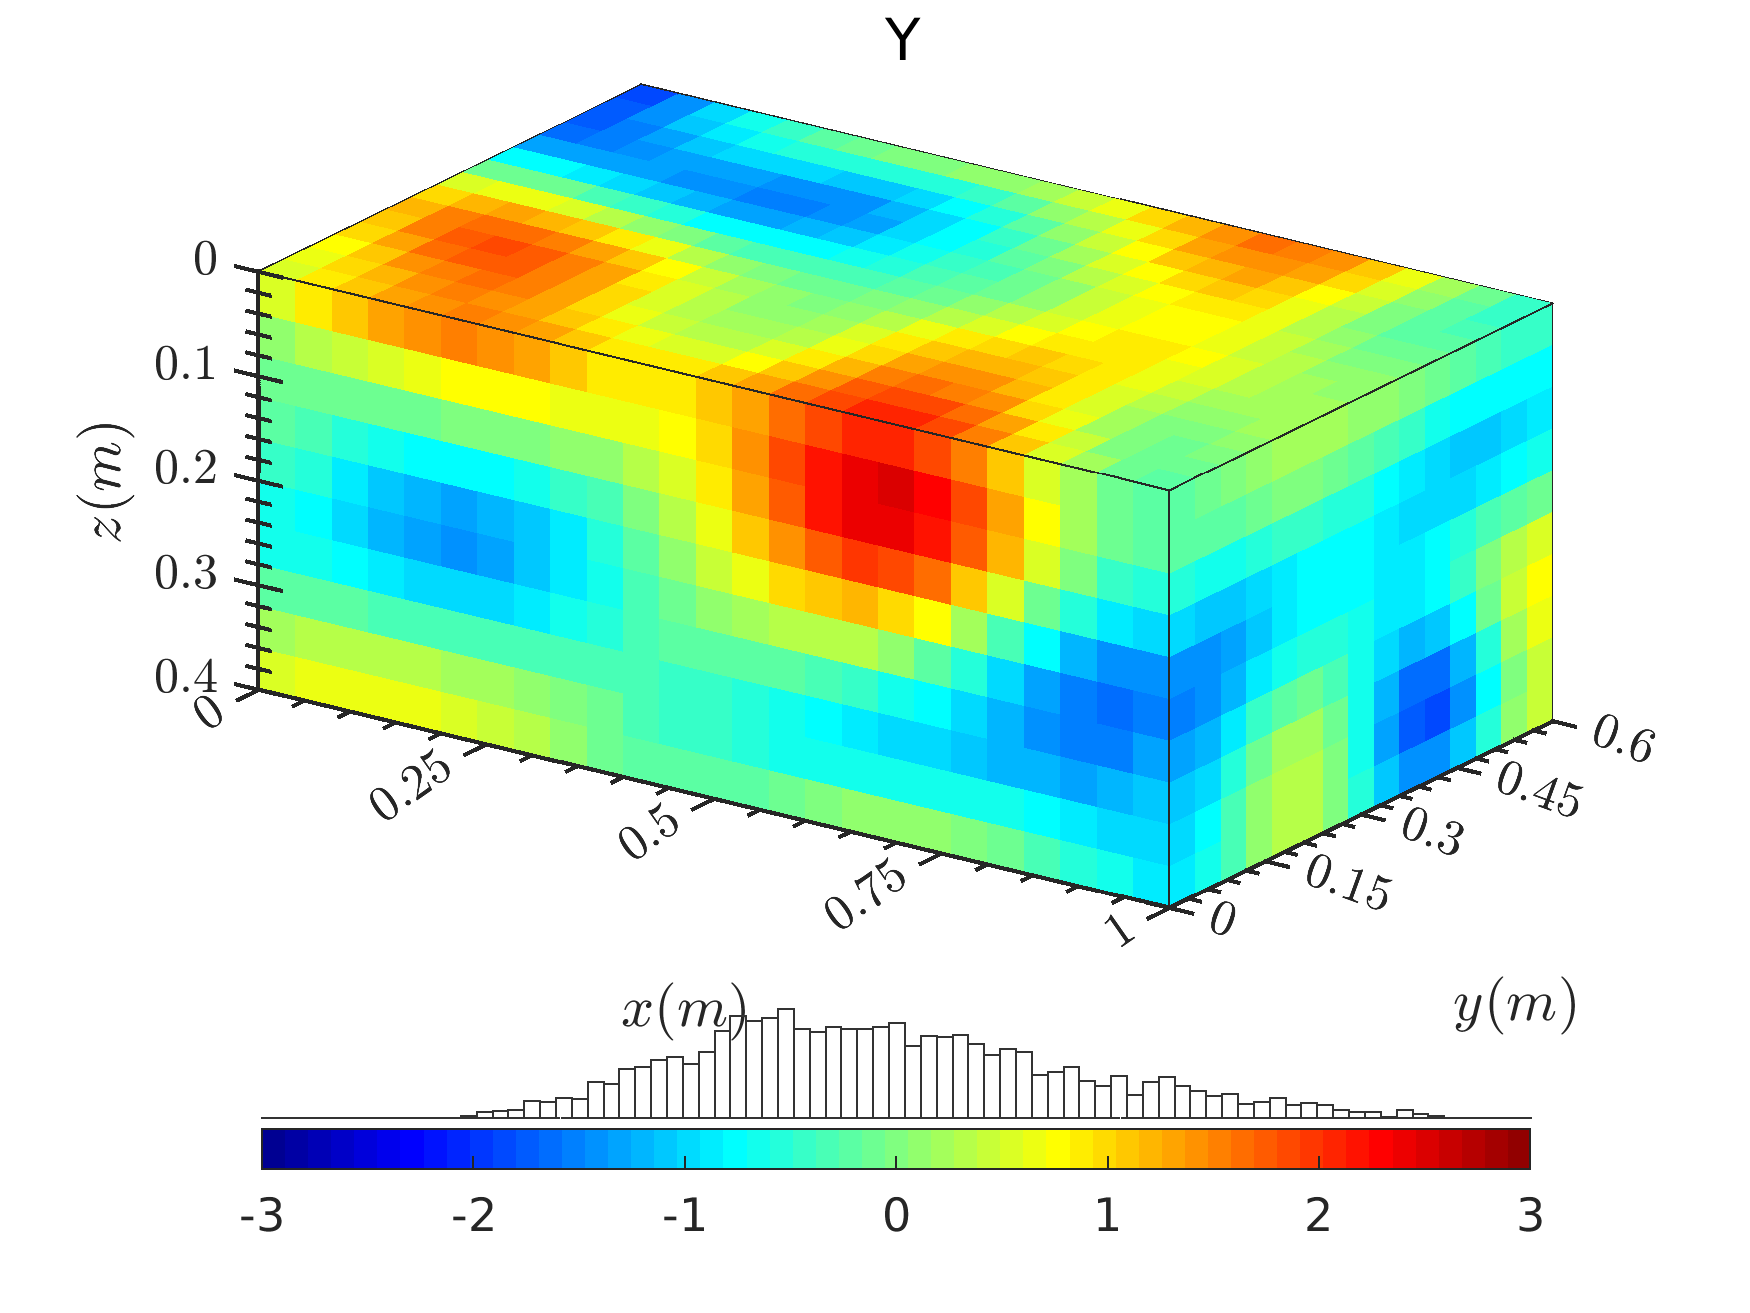
\includegraphics[scale=0.5]{./figuras/Y_sexpUNCOND_0.png}}
 \subfigure[]{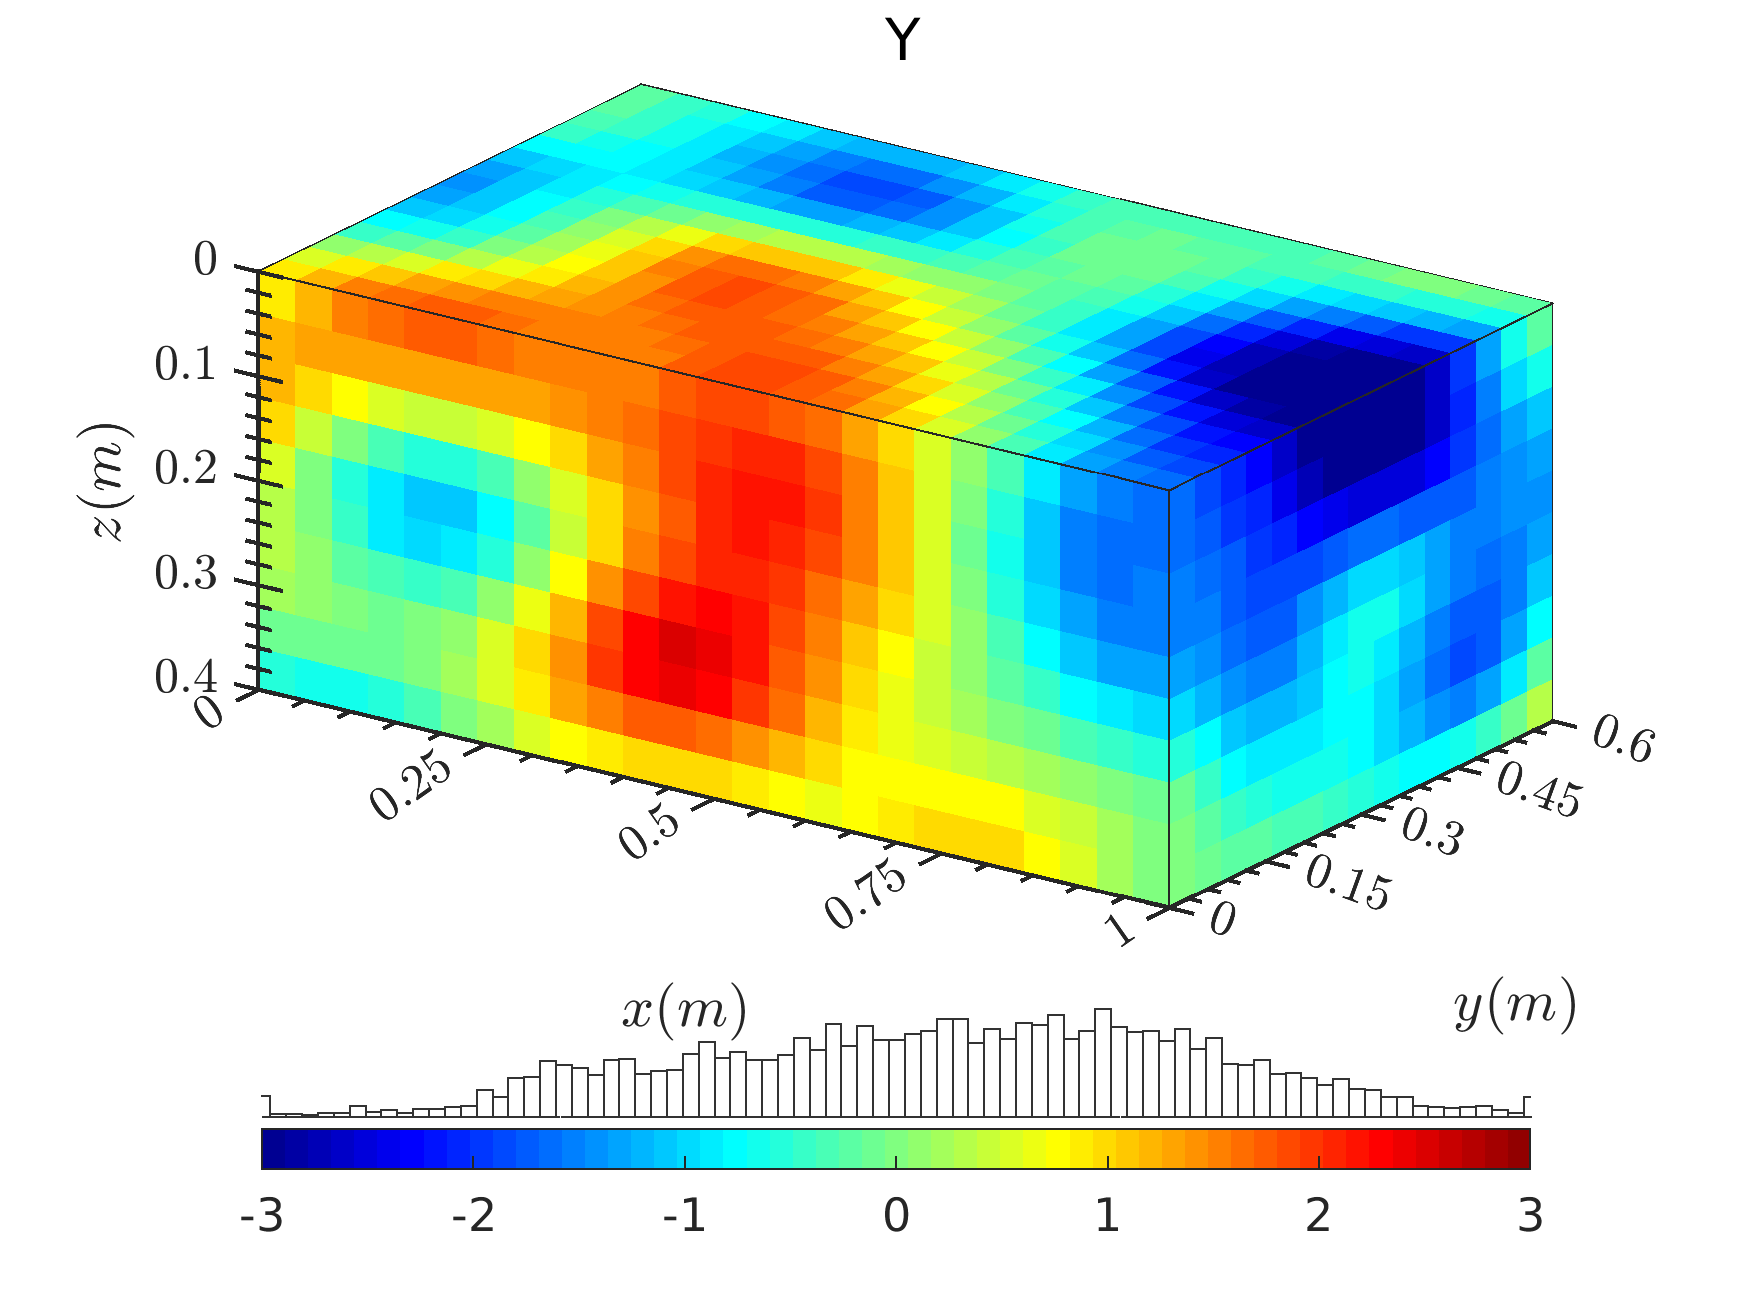
\includegraphics[scale=0.5]{./figuras/Y_sexpUNCOND_1.png}}
 \subfigure[]{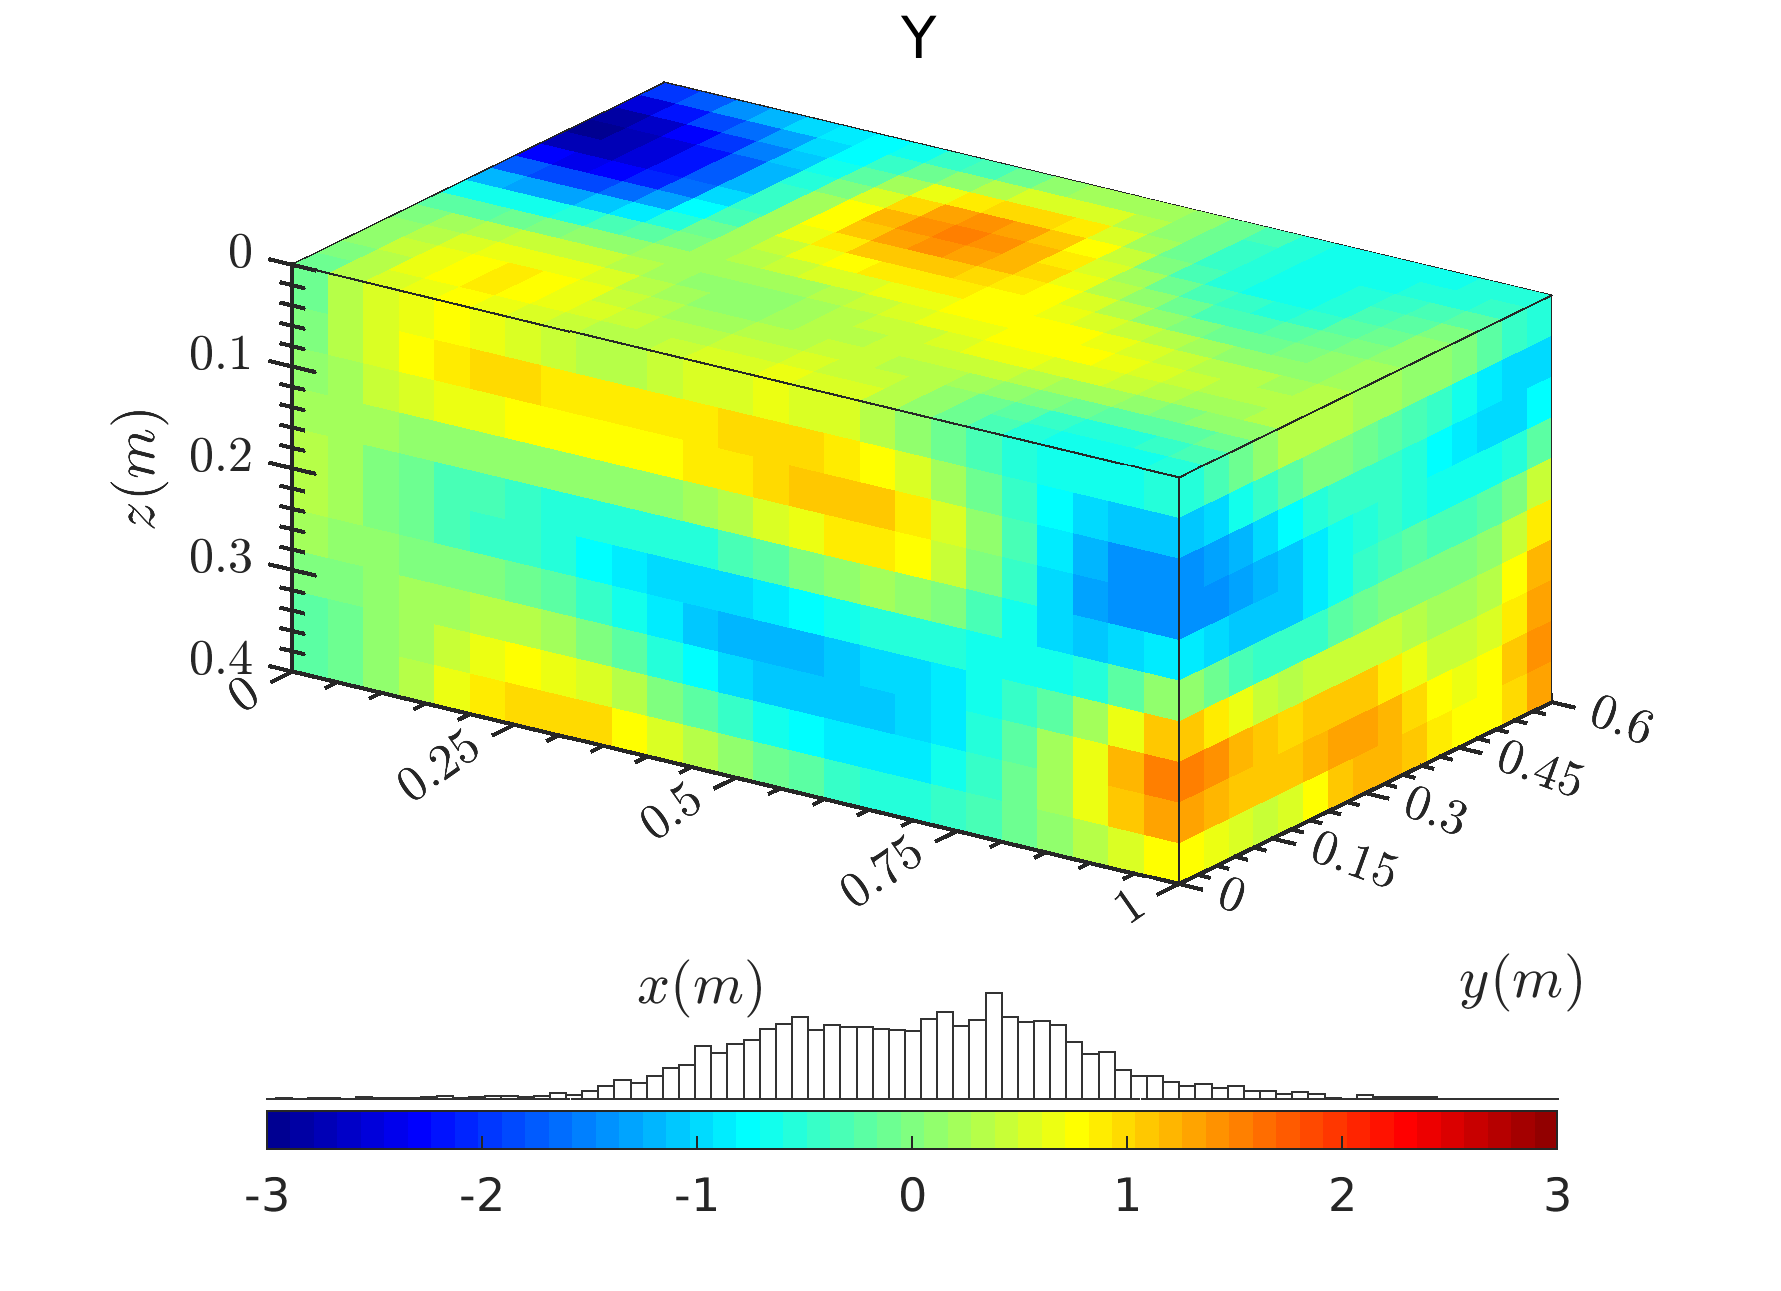
\includegraphics[scale=0.5]{./figuras/Y_sexpUNCOND_2.png}}
 \subfigure[]{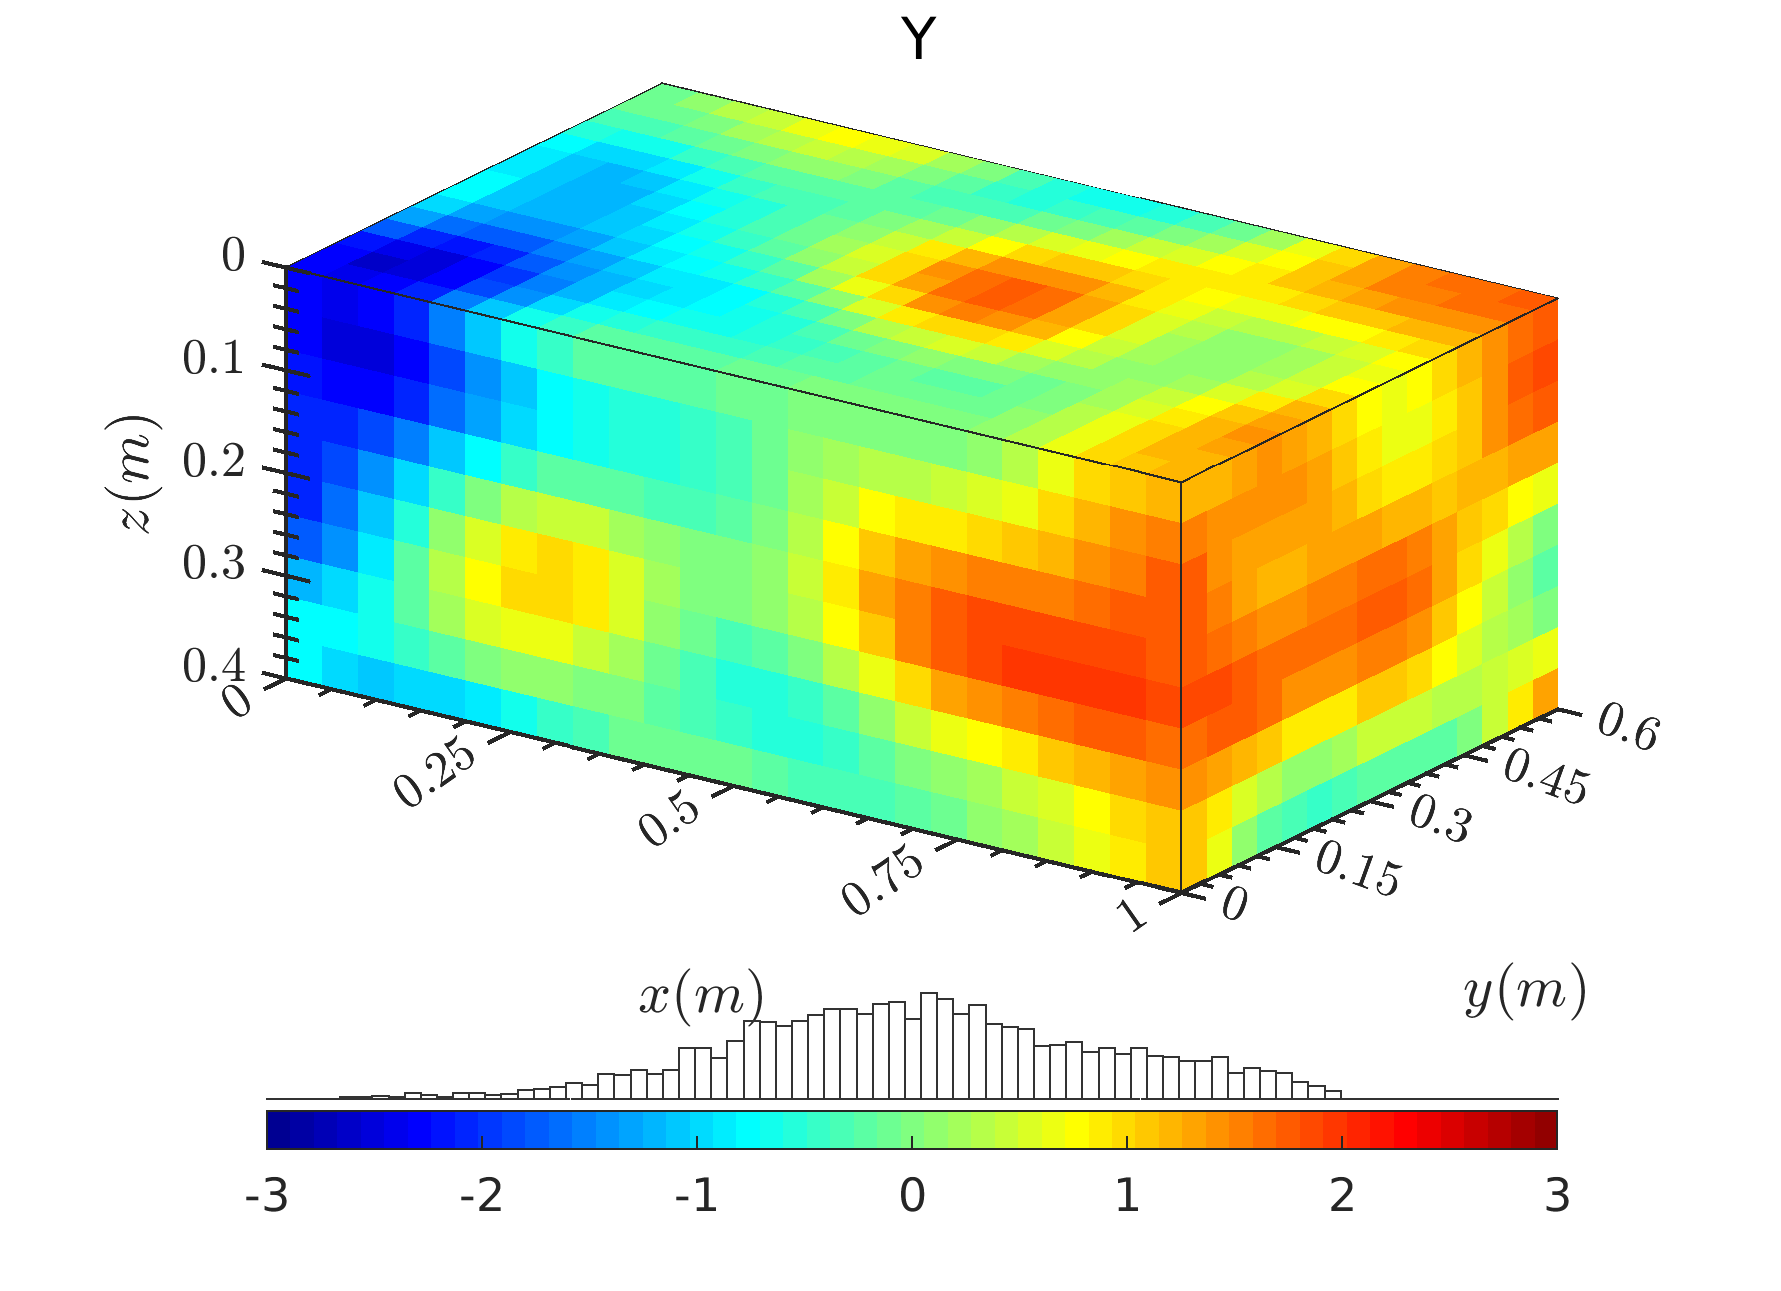
\includegraphics[scale=0.5]{./figuras/Y_sexpUNCOND_3.png}}
 \caption{Realizations of random fields with squared exponential covariance (\eq{eq-squarecov}).}
 \label{fig-uncondFields}
\end{figure}


\fig{fig-uncondCov} shows the computed covariance function obtained with 2000 realizations. 
The models obtained (red line) by fitting the computed points are in excellent agreement with the theoretical model (\eq{eq-squarecov}).

\begin{figure}[H]
 \centering
 \subfigure[Direction $x$]{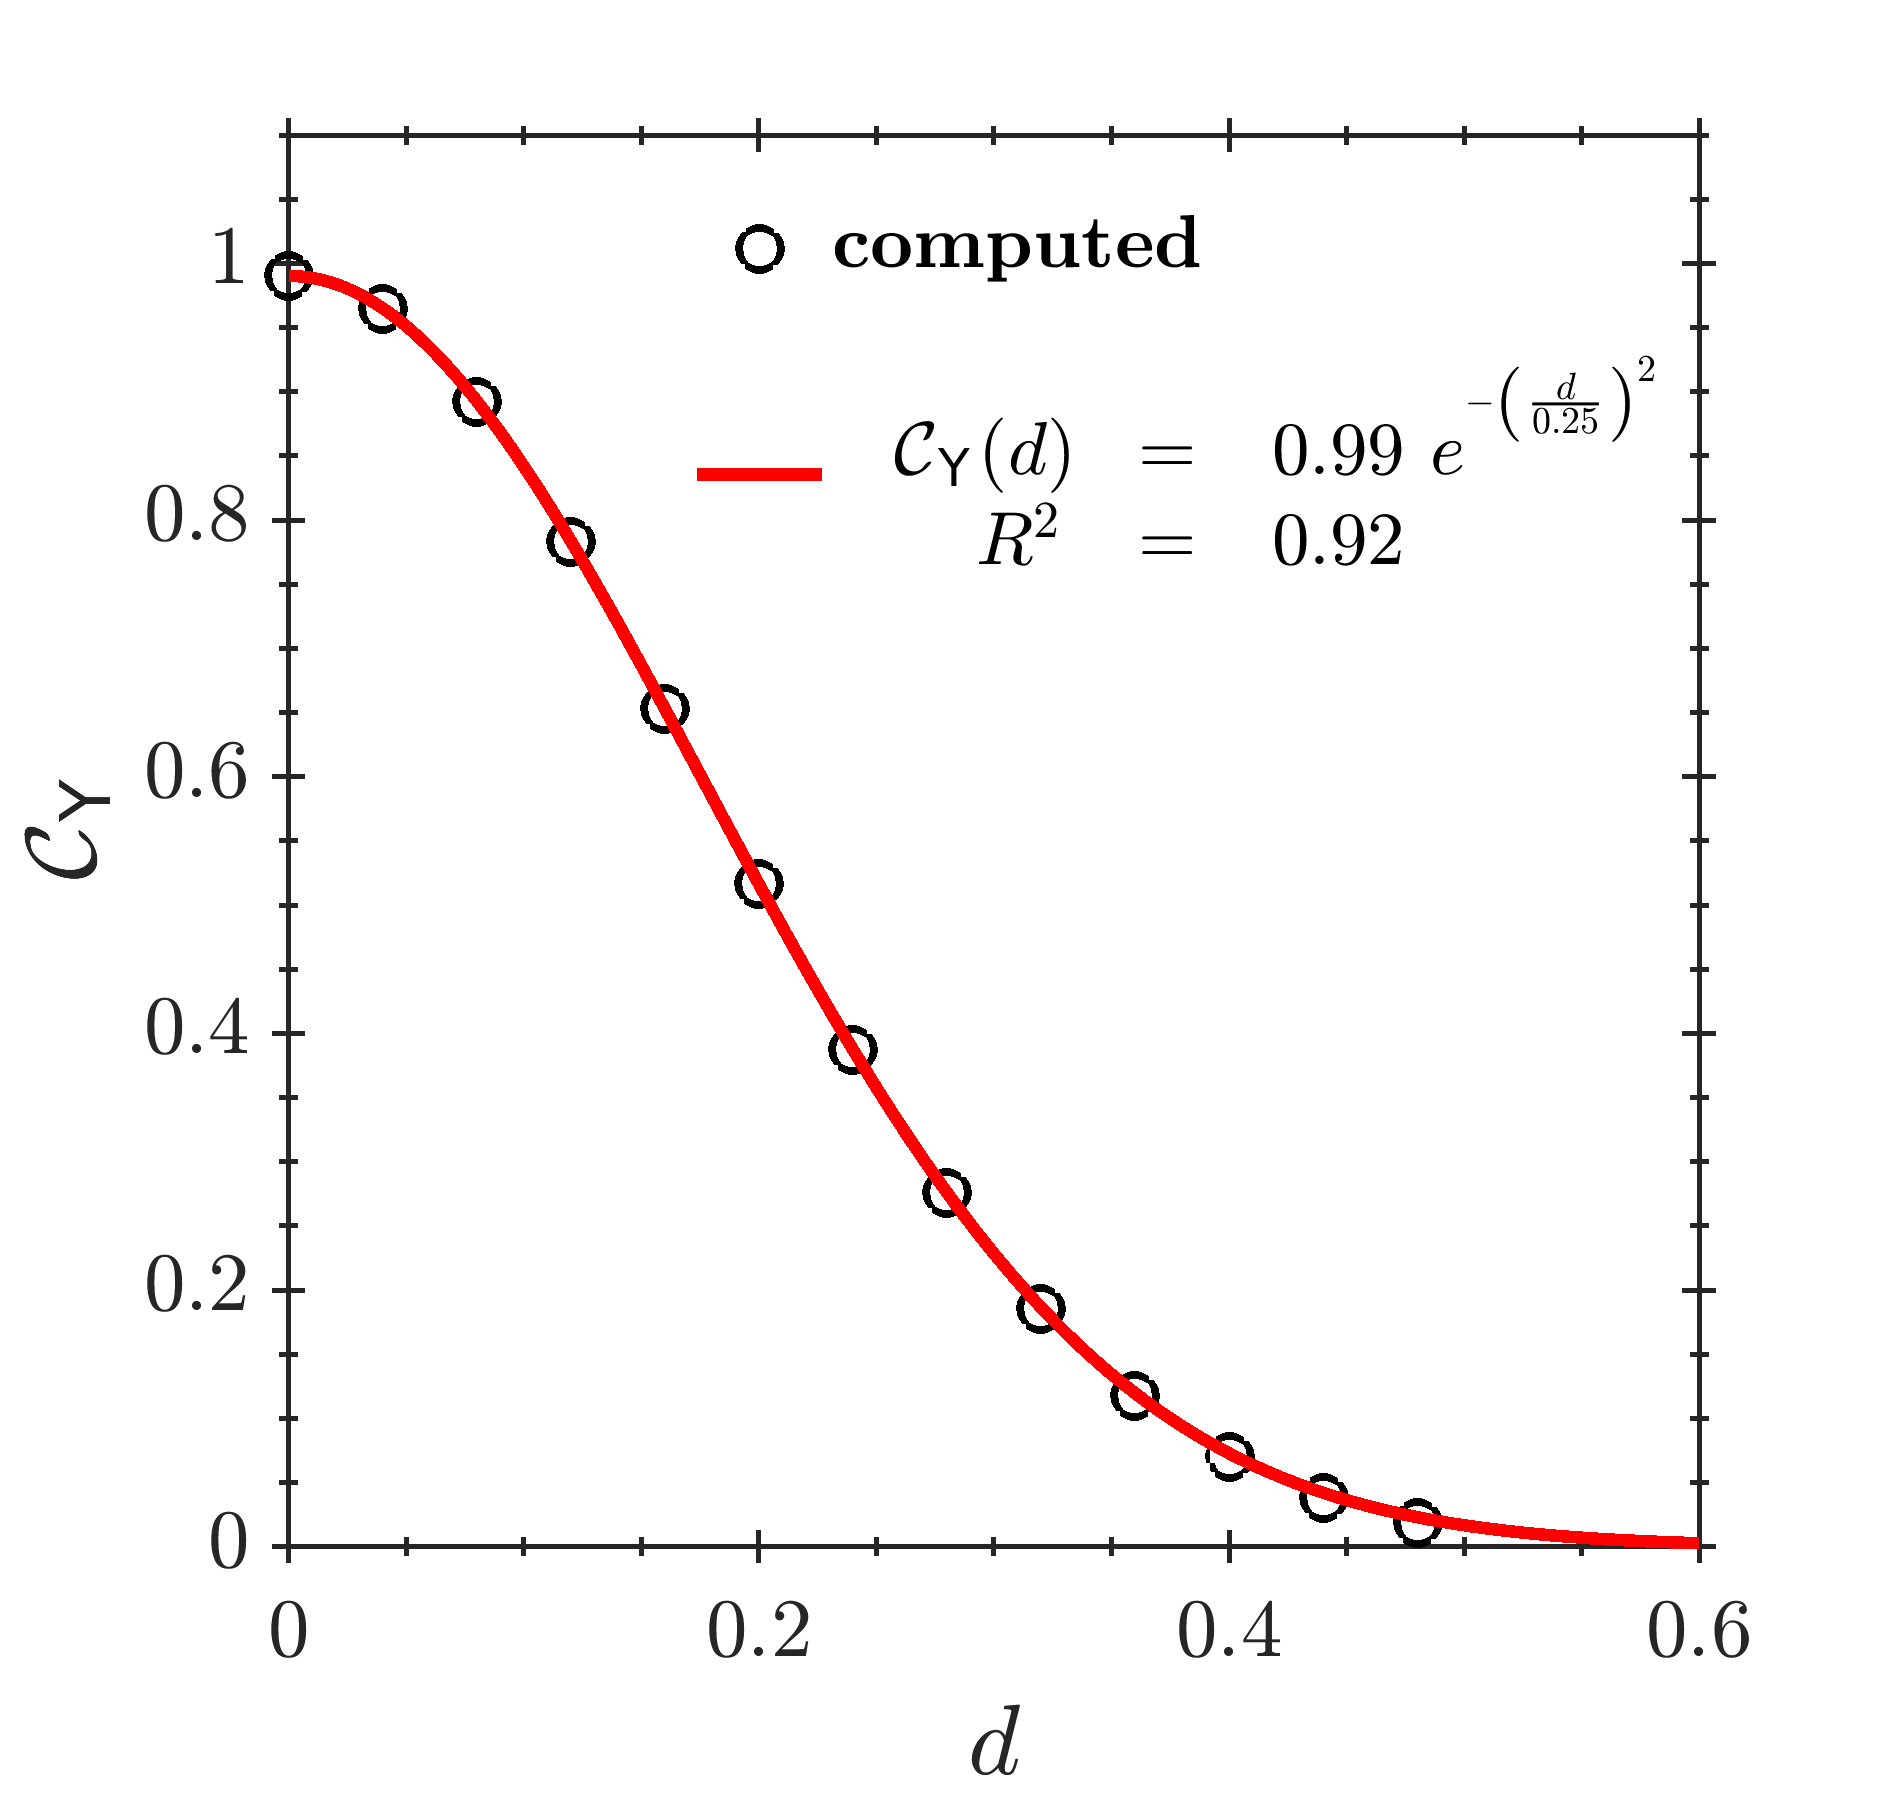
\includegraphics[scale = 0.325]{./figuras/e_gsexp_1x0_6x0_4_25x15x10_0-2x0-2x0-1_5000_Yx.png}}
 \subfigure[Direction $y$]{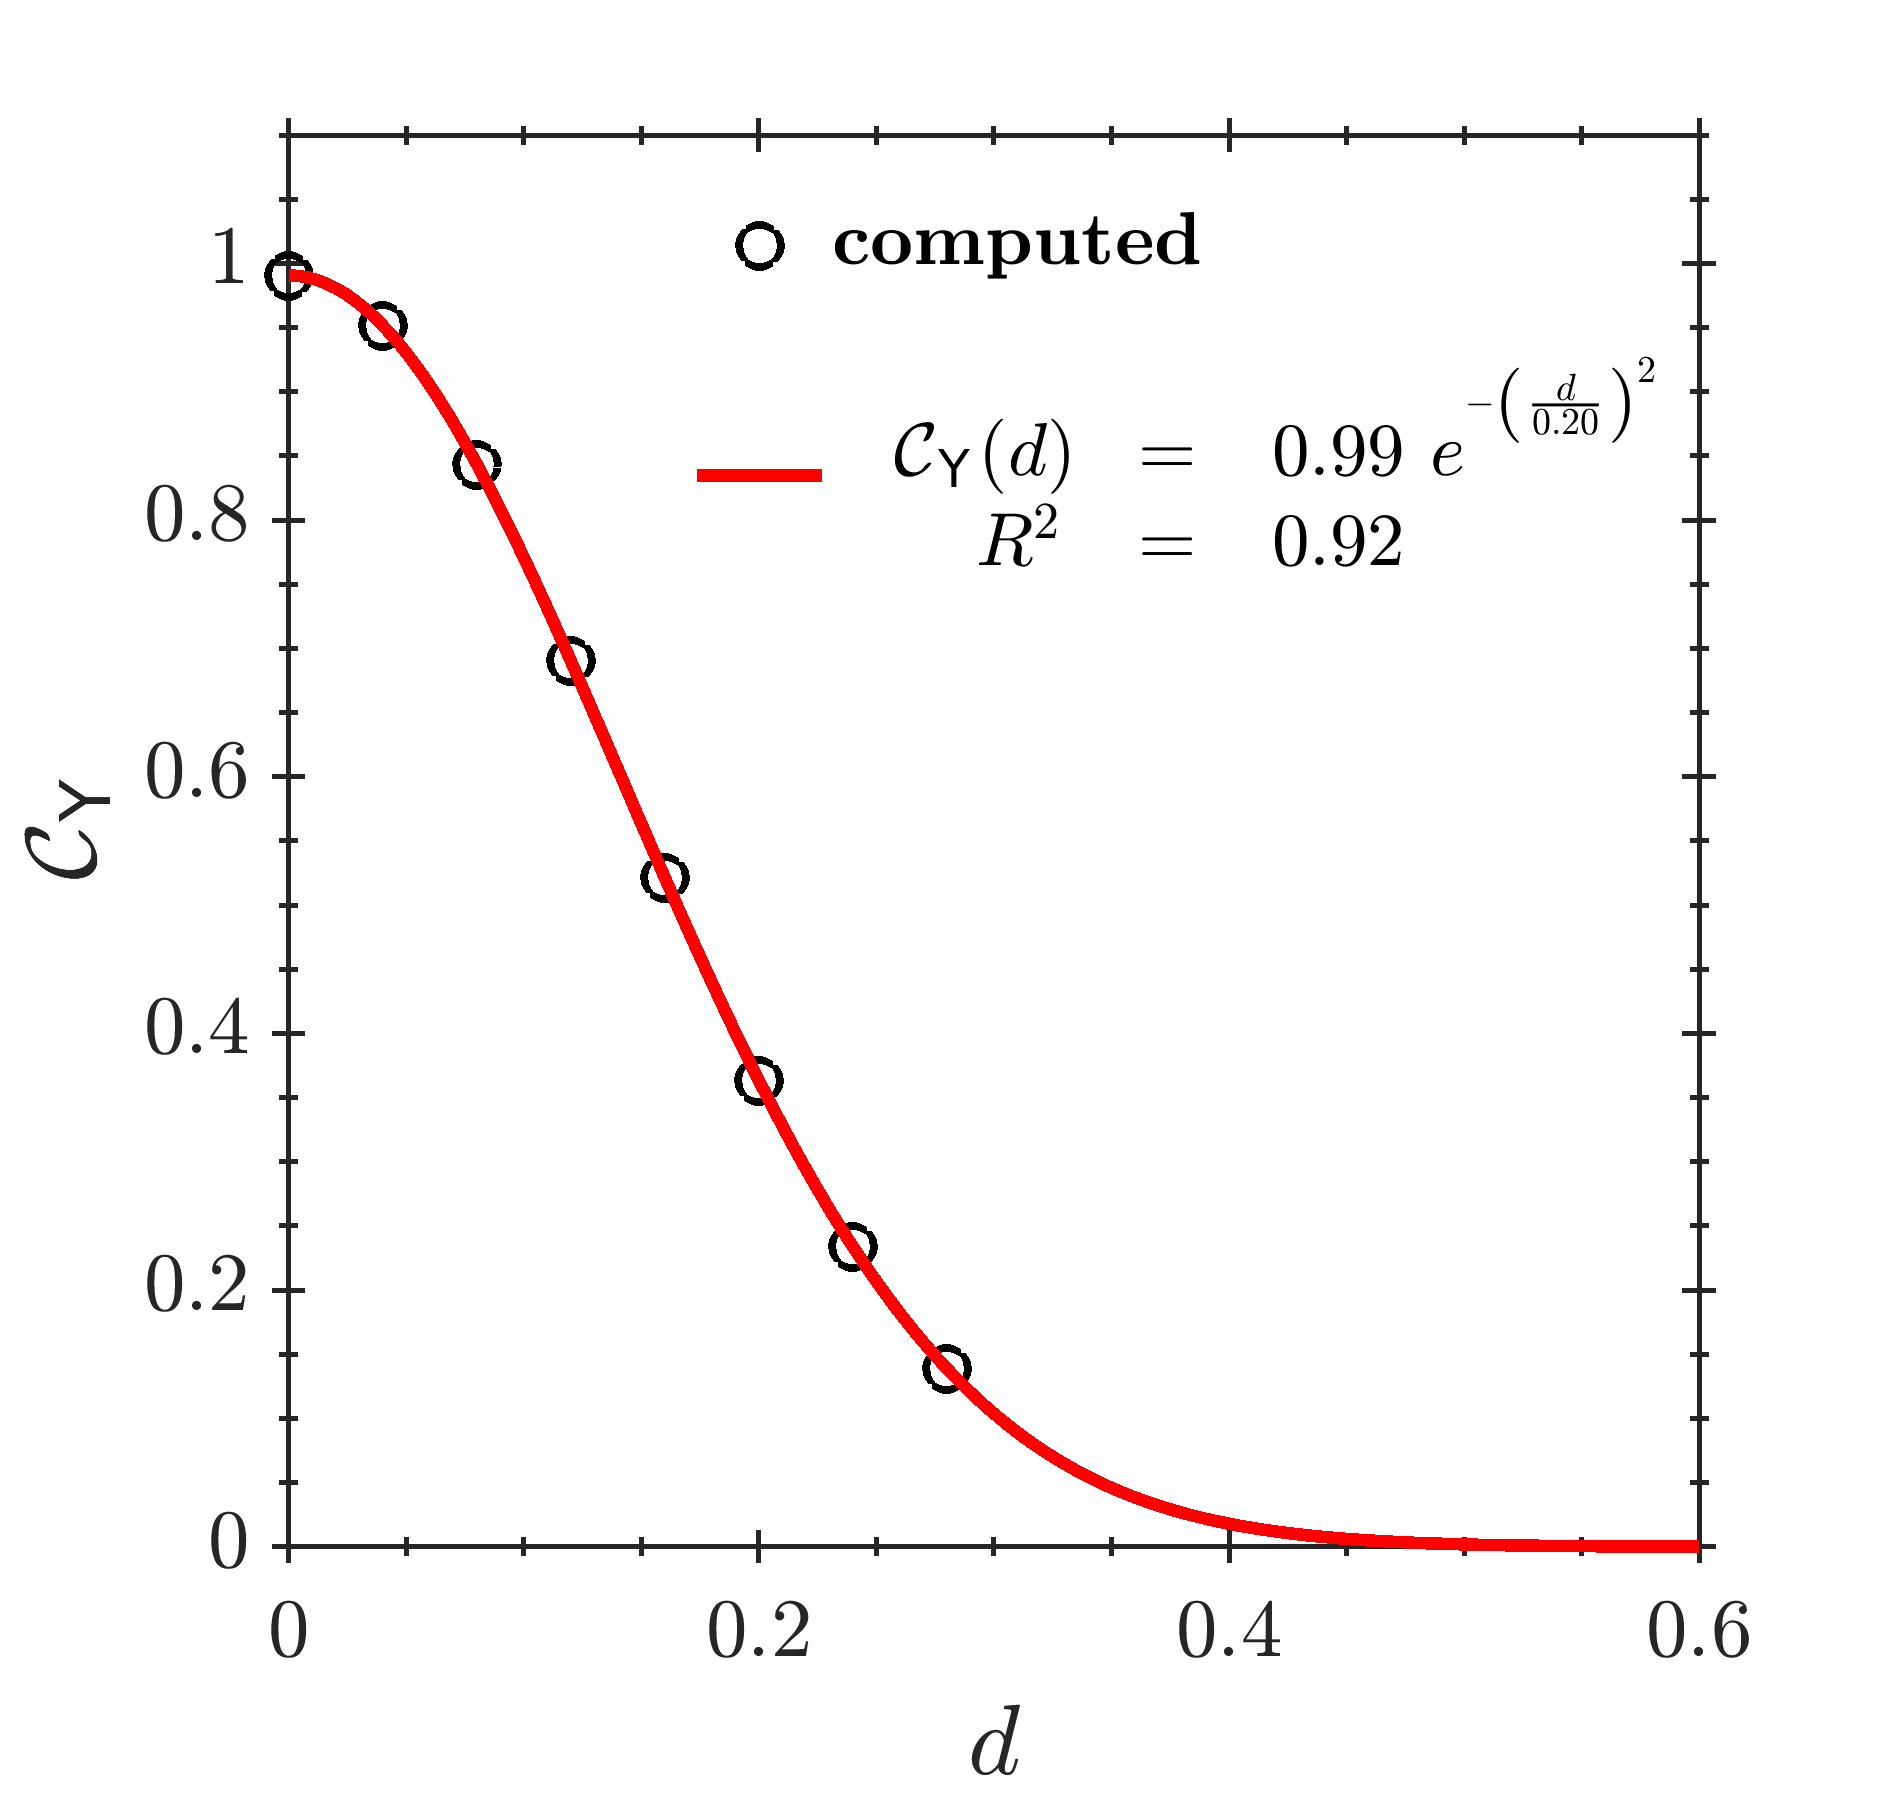
\includegraphics[scale = 0.325]{./figuras/e_gsexp_1x0_6x0_4_25x15x10_0-2x0-2x0-1_5000_Yy.png}}
 \subfigure[Direction $z$]{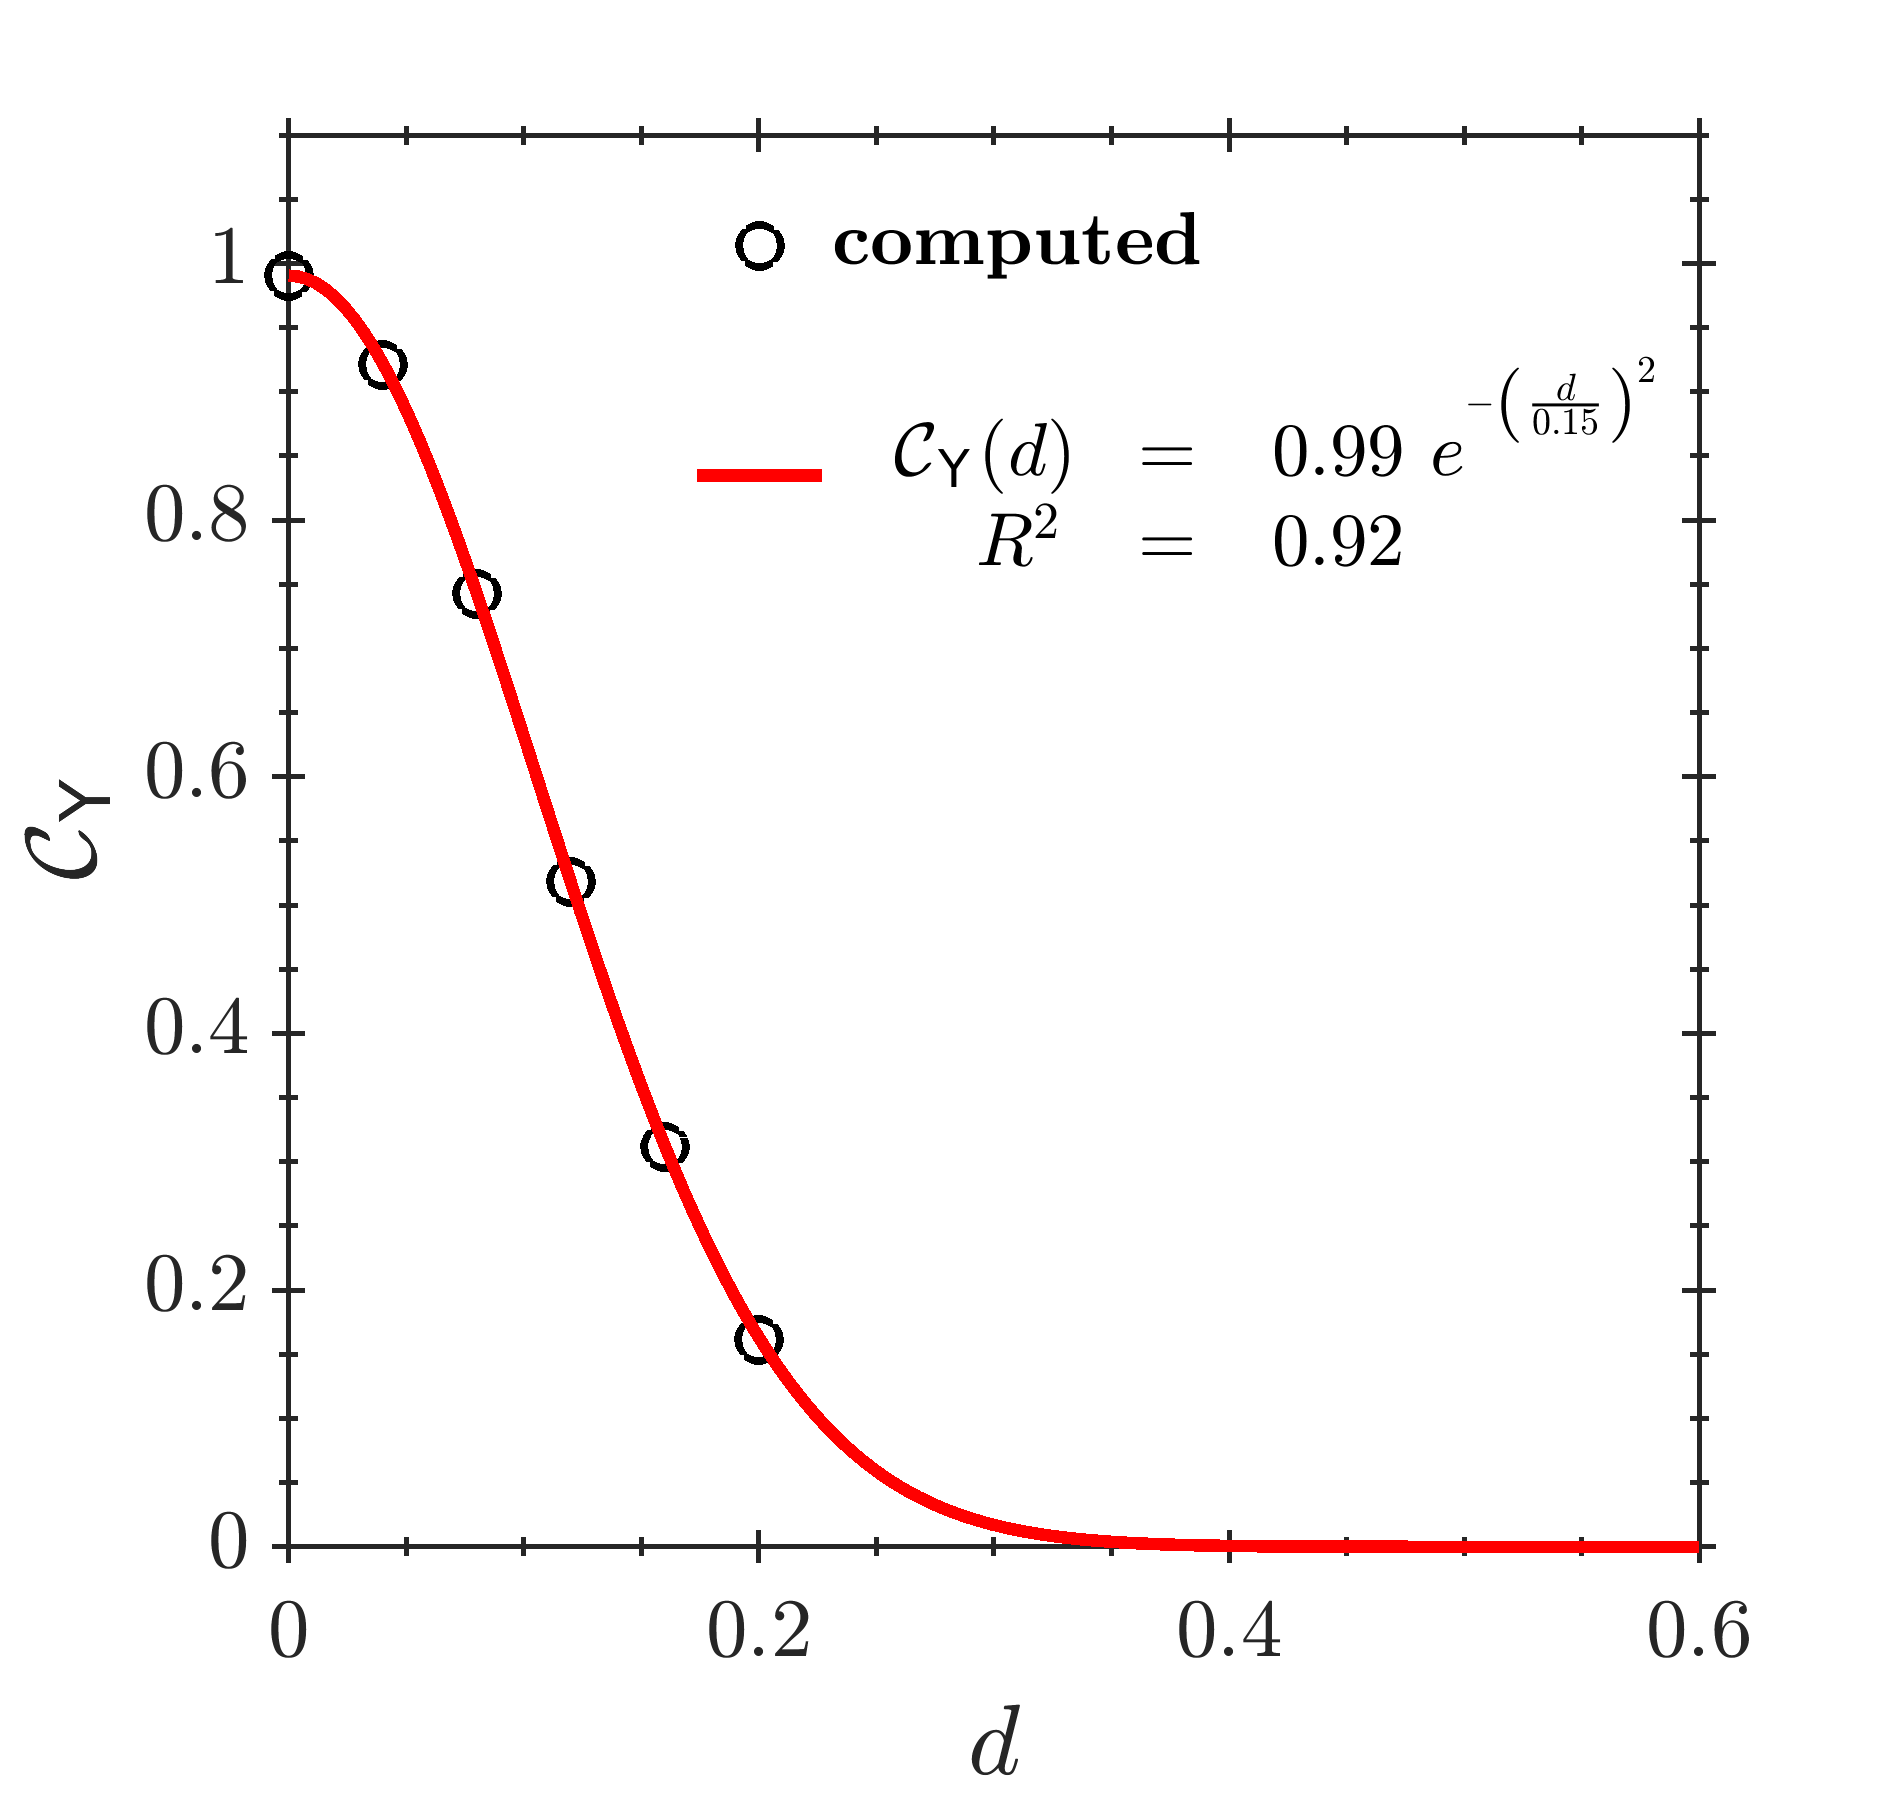
\includegraphics[scale = 0.325]{./figuras/e_gsexp_1x0_6x0_4_25x15x10_0-2x0-2x0-1_5000_Yz.png}}
 \caption{Covariance as function of the lag distance $d=\lVert \vx - \vy \rVert$, computed with an ensamble of 2000 unconditioned fields.}
 \label{fig-uncondCov}
\end{figure}

%%%%%%%%%%%%%%%%%%%%%%%%%%%%%%%%%%%%%%%%%%%%%%%%%%%%%%%%%%%%%%%%%%
\subsubsection{Conditioned}

In this section, an experiment similar to the previous one is conducted, however, the fields are conditioned at four points, as shown in the \tab{tab-cond}.

% \begin{table}[H]
%  \caption{Conditioned points}\label{tab-cond}
% \begin{center}
% \begin{tabular}{cccc}\hline\hline
% $x$ & $y$ & $z$ & $\Y\fx$\\ \hline
% 0.125 & 0.025 & 0.375 & 1.000\\
% 0.575 & 0.025 & 0.125 & 1.000\\
% 0.975 & 0.175 & 0.225 & -1.000\\
% 0.975 & 0.525 & 0.175 & -1.000\\ \hline\hline
% \end{tabular}
% \end{center}
% \end{table}

{%
\begin{table}[H]
 \caption{Conditioned points}\label{tab-cond}
\newcommand{\mc}[3]{\multicolumn{#1}{#2}{#3}}
\begin{center}
\begin{tabular}{cllc}
\hline\hline
\mc{3}{c}{{Point $\vx$}} & \\
$x$ & \mc{1}{c}{$y$} & \mc{1}{c}{$z$} & $\Y\fx$\\ \hline
0.125 & \mc{1}{c}{0.025} & \mc{1}{c}{0.375} & 1.000\\
0.575 & \mc{1}{c}{0.025} & \mc{1}{c}{0.125} & 1.000\\
0.975 & \mc{1}{c}{0.175} & \mc{1}{c}{0.225} & -1.000\\
0.975 & \mc{1}{c}{0.525} & \mc{1}{c}{0.175} & -1.000\\ \hline\hline
\end{tabular}
\end{center}
\end{table}
}%


In \fig{fig-condFields} two realizations of the fields are presented and the cubes show the conditioned points.

\begin{figure}[H]
 \centering
 \subfigure[]{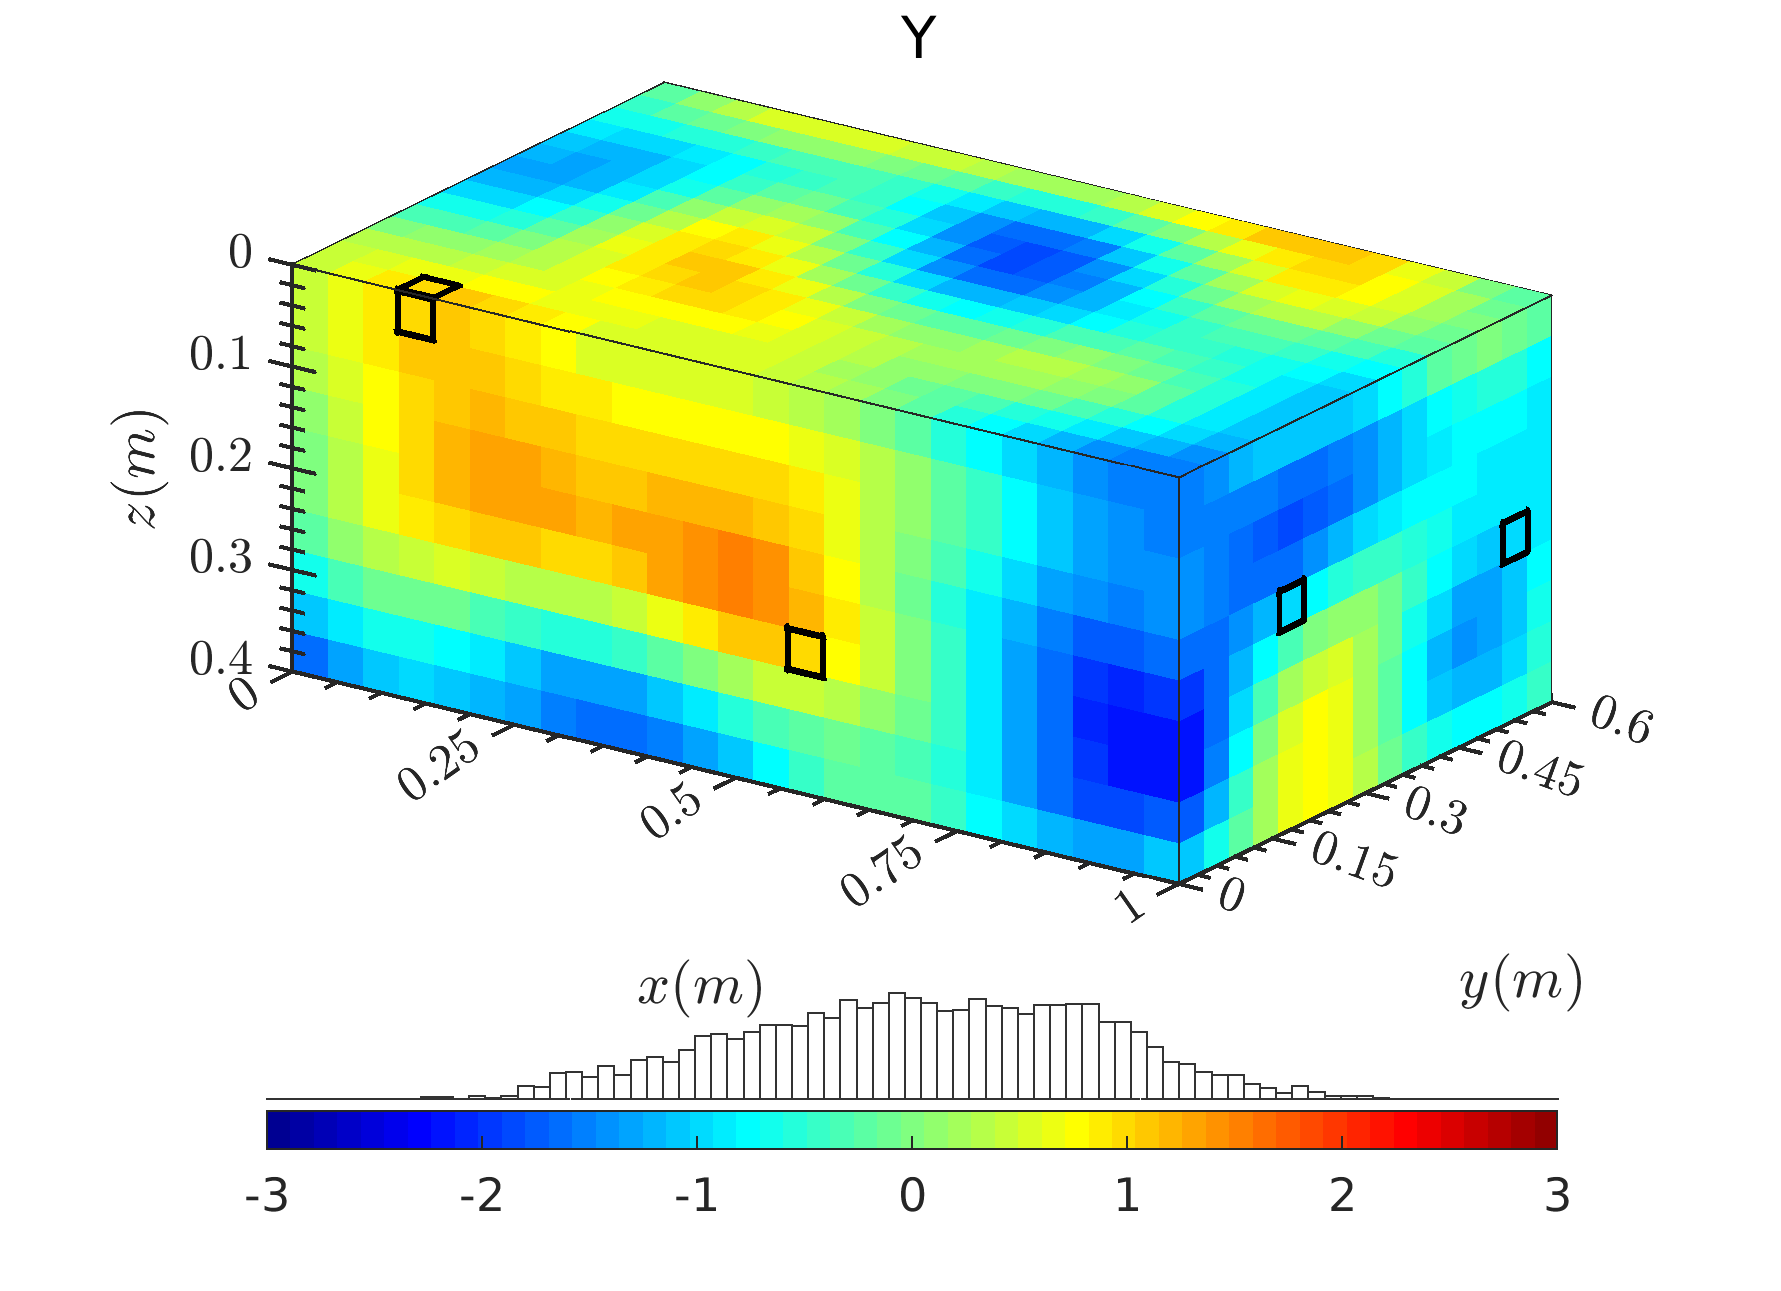
\includegraphics[scale=0.5]{./figuras/Y_sexpCOND_0.png}}
 \subfigure[]{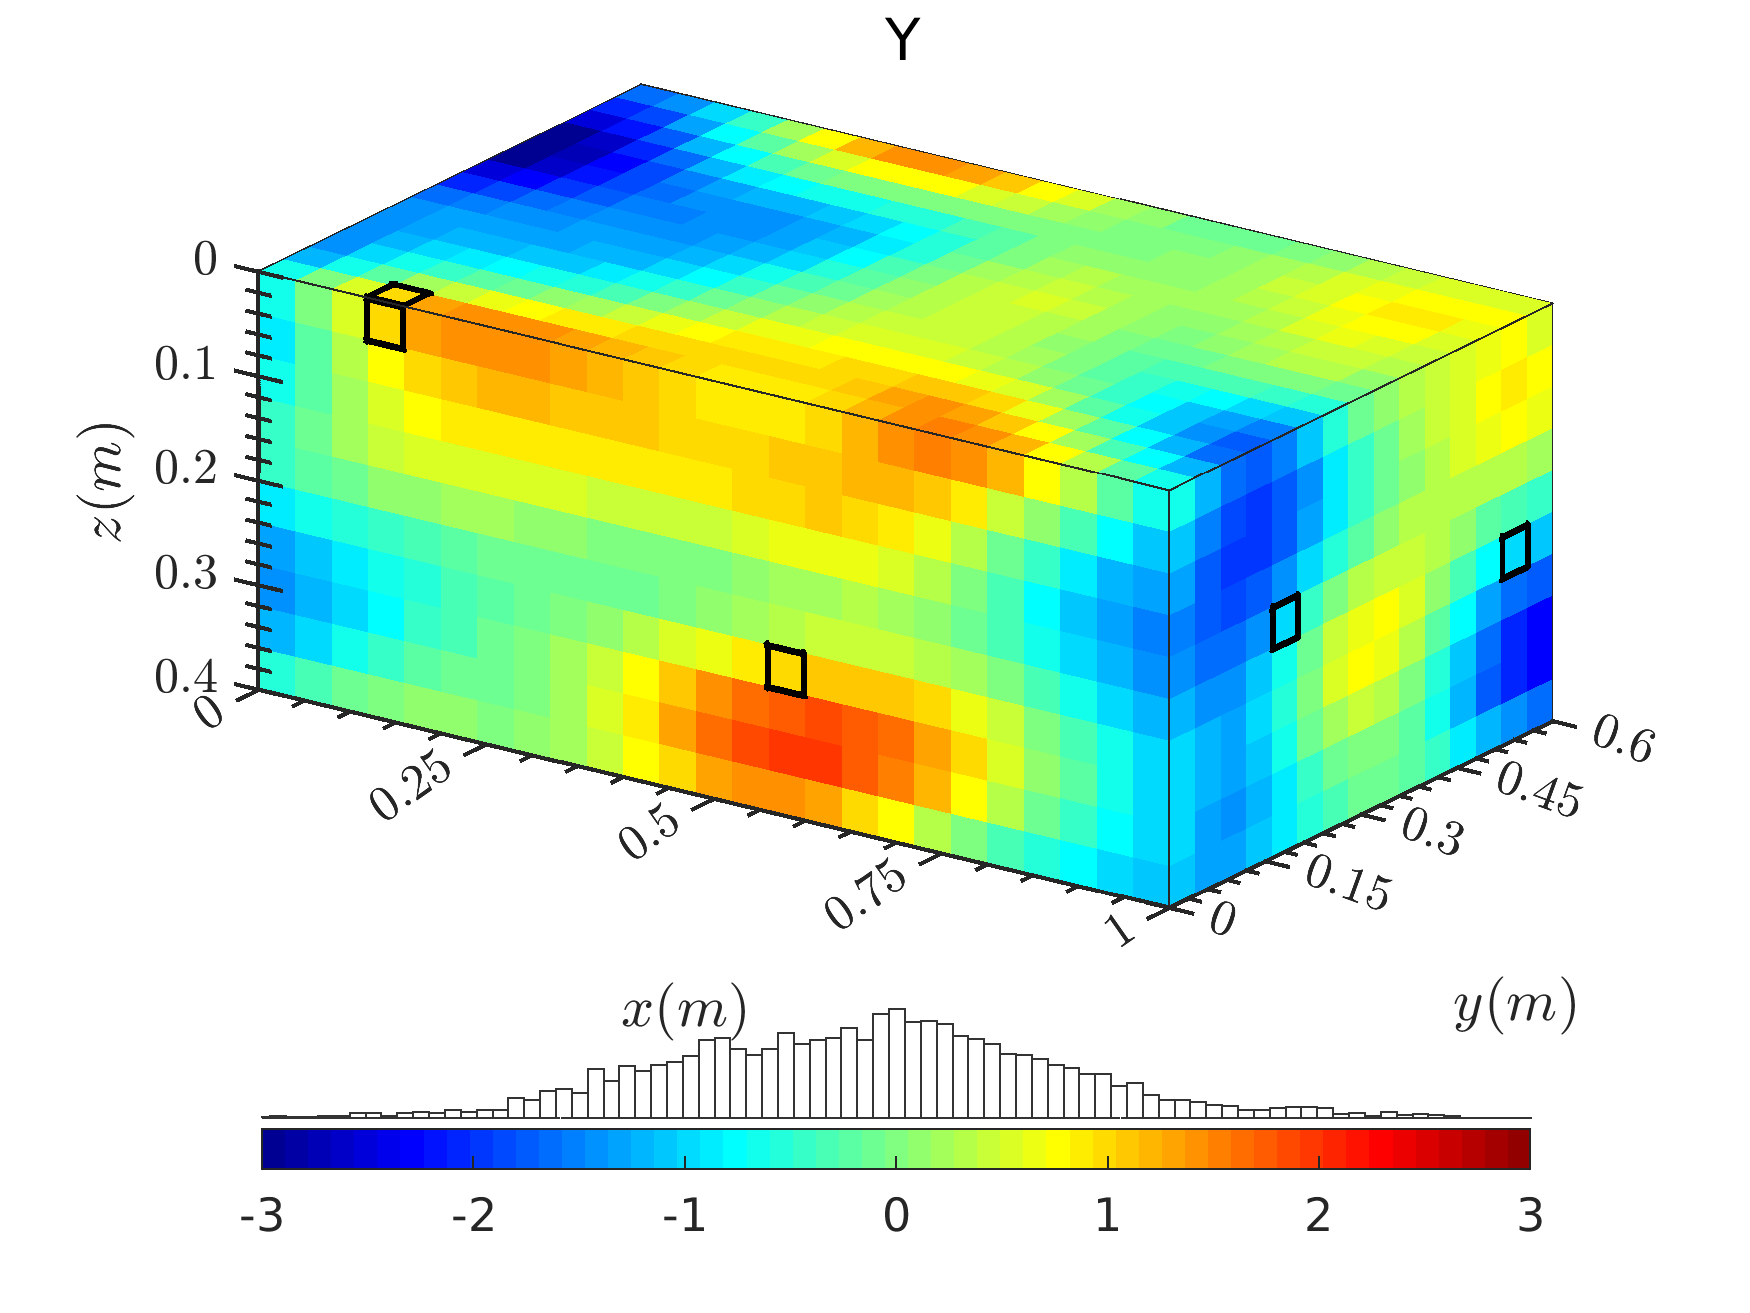
\includegraphics[scale=0.5]{./figuras/Y_sexpCOND_1.png}}
 \subfigure[]{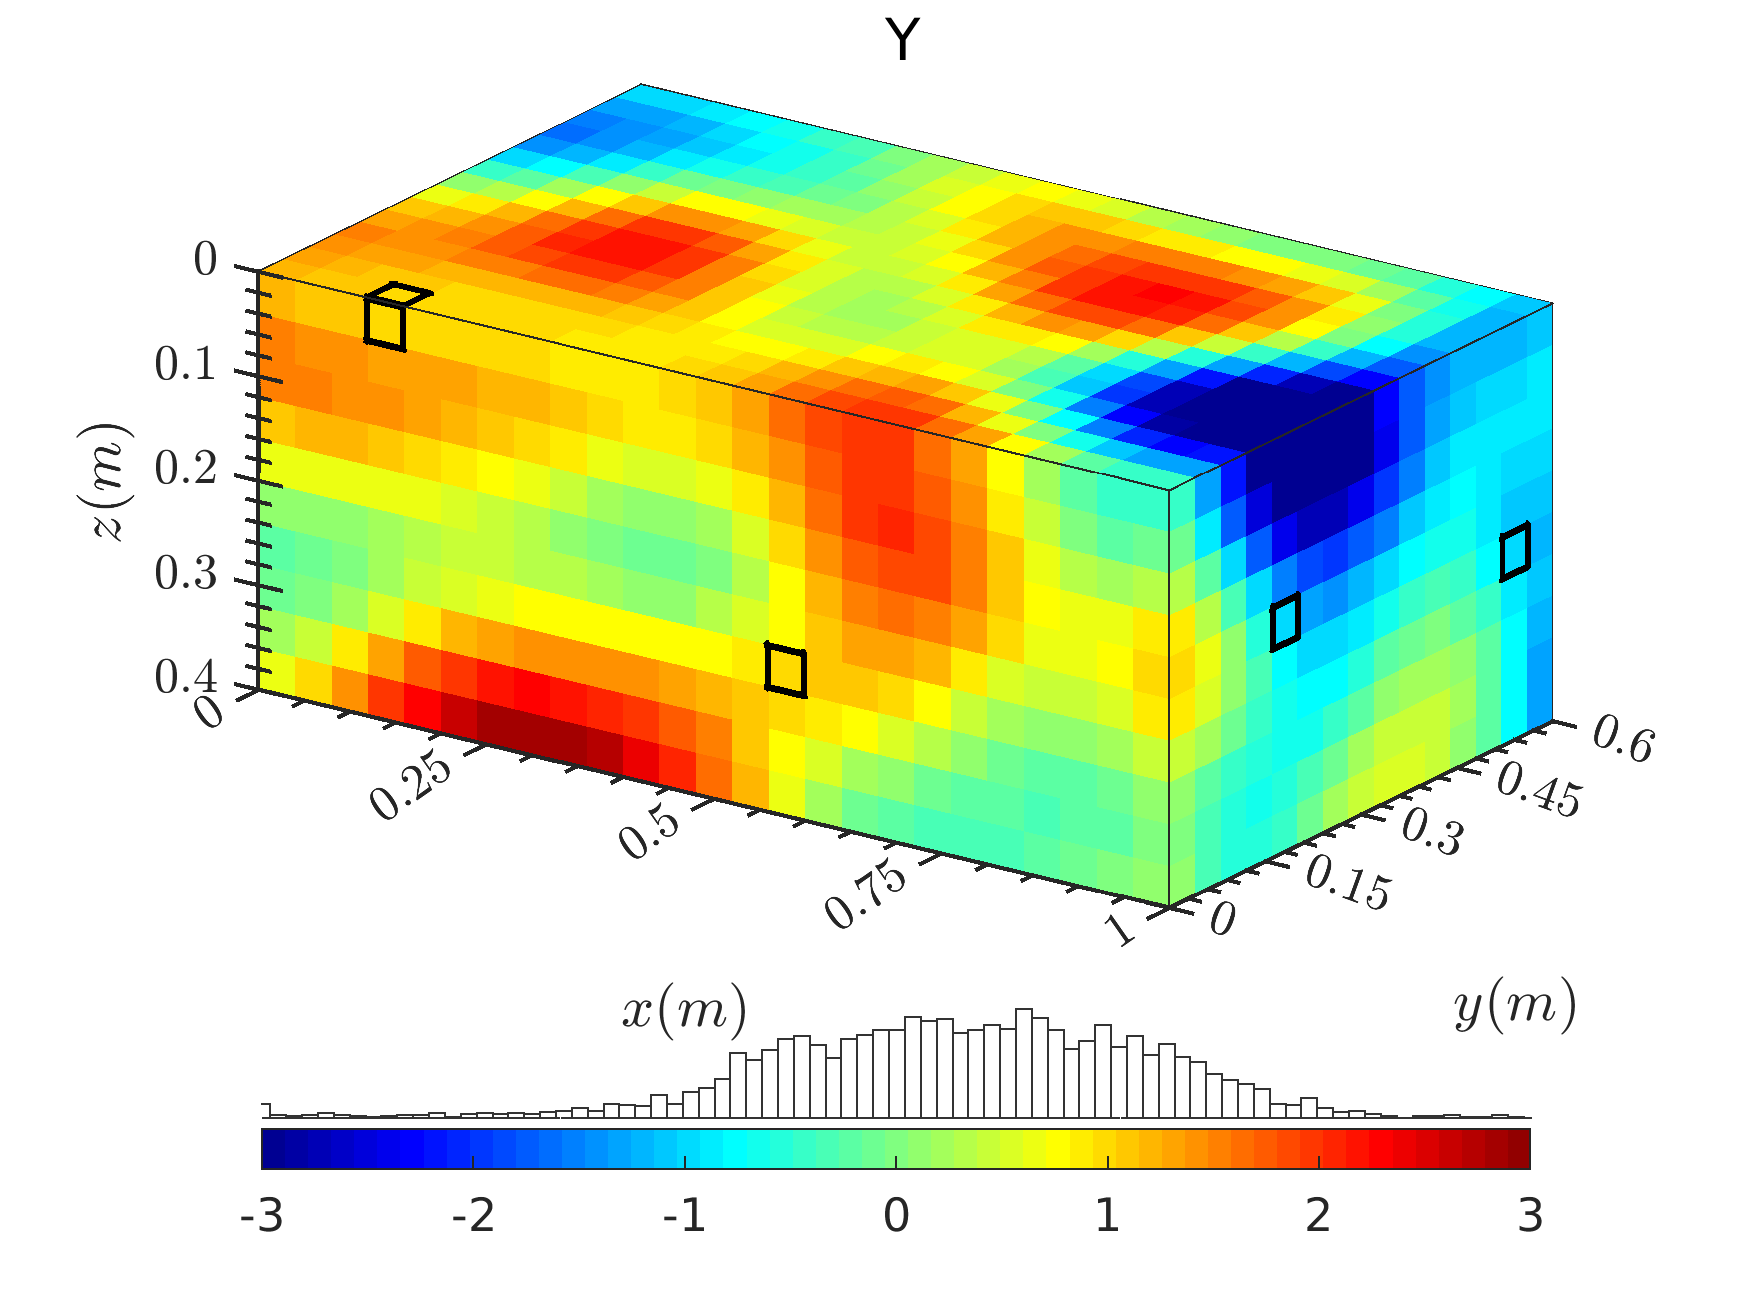
\includegraphics[scale=0.5]{./figuras/Y_sexpCOND_2.png}}
 \subfigure[]{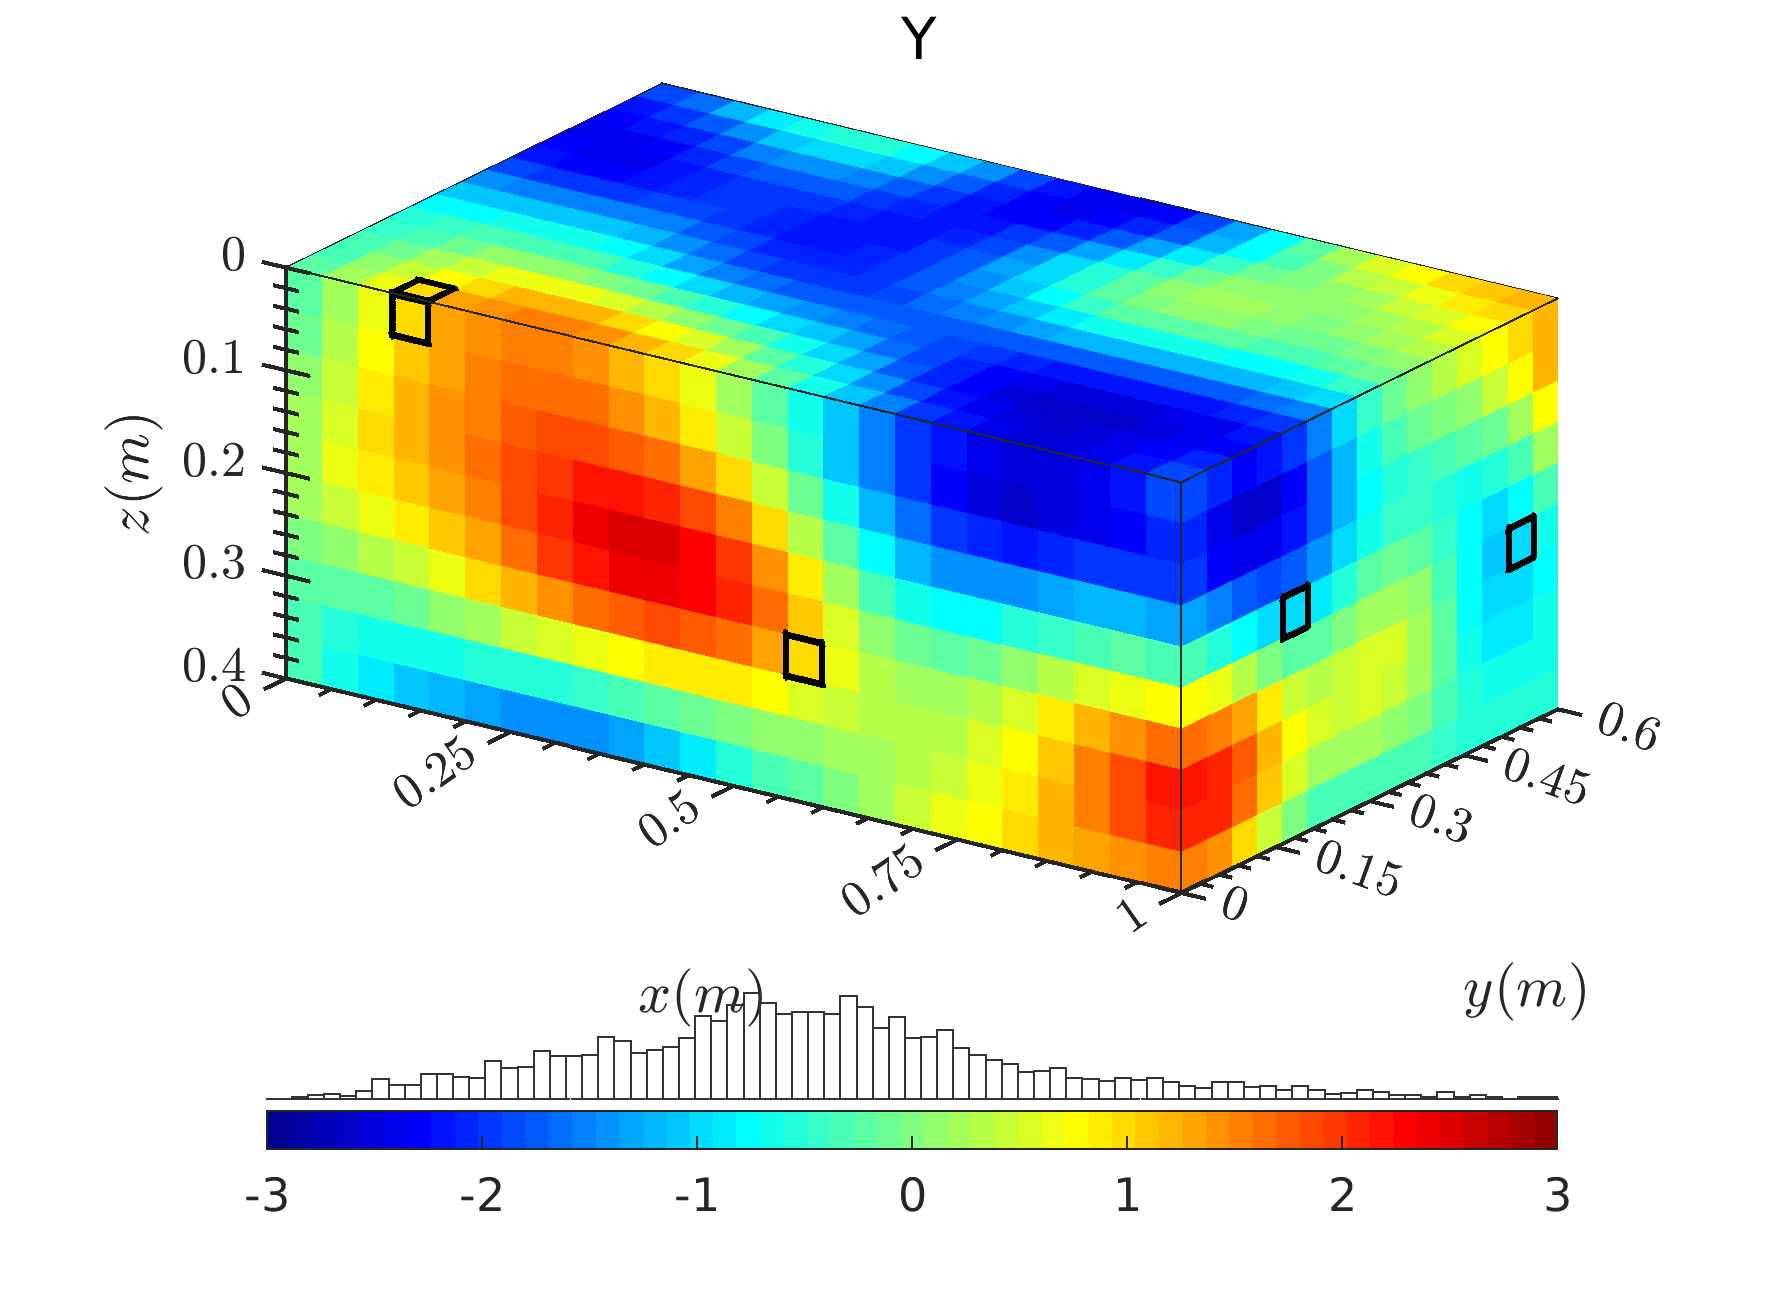
\includegraphics[scale=0.5]{./figuras/Y_sexpCOND_3.png}}
 \caption{Realizations of random fields with squared exponential covariance (\eq{eq-squarecov}).}
 \label{fig-condFields}
\end{figure}

\fig{fig-uncondCov} shows the computed covariance function obtained with 2000 realizations. 
The models obtained (red line) by fitting the computed points are in excellent agreement with the theoretical model (\eq{eq-squarecov}).

\begin{figure}[H]
 \centering
 \subfigure[Direction $x$]{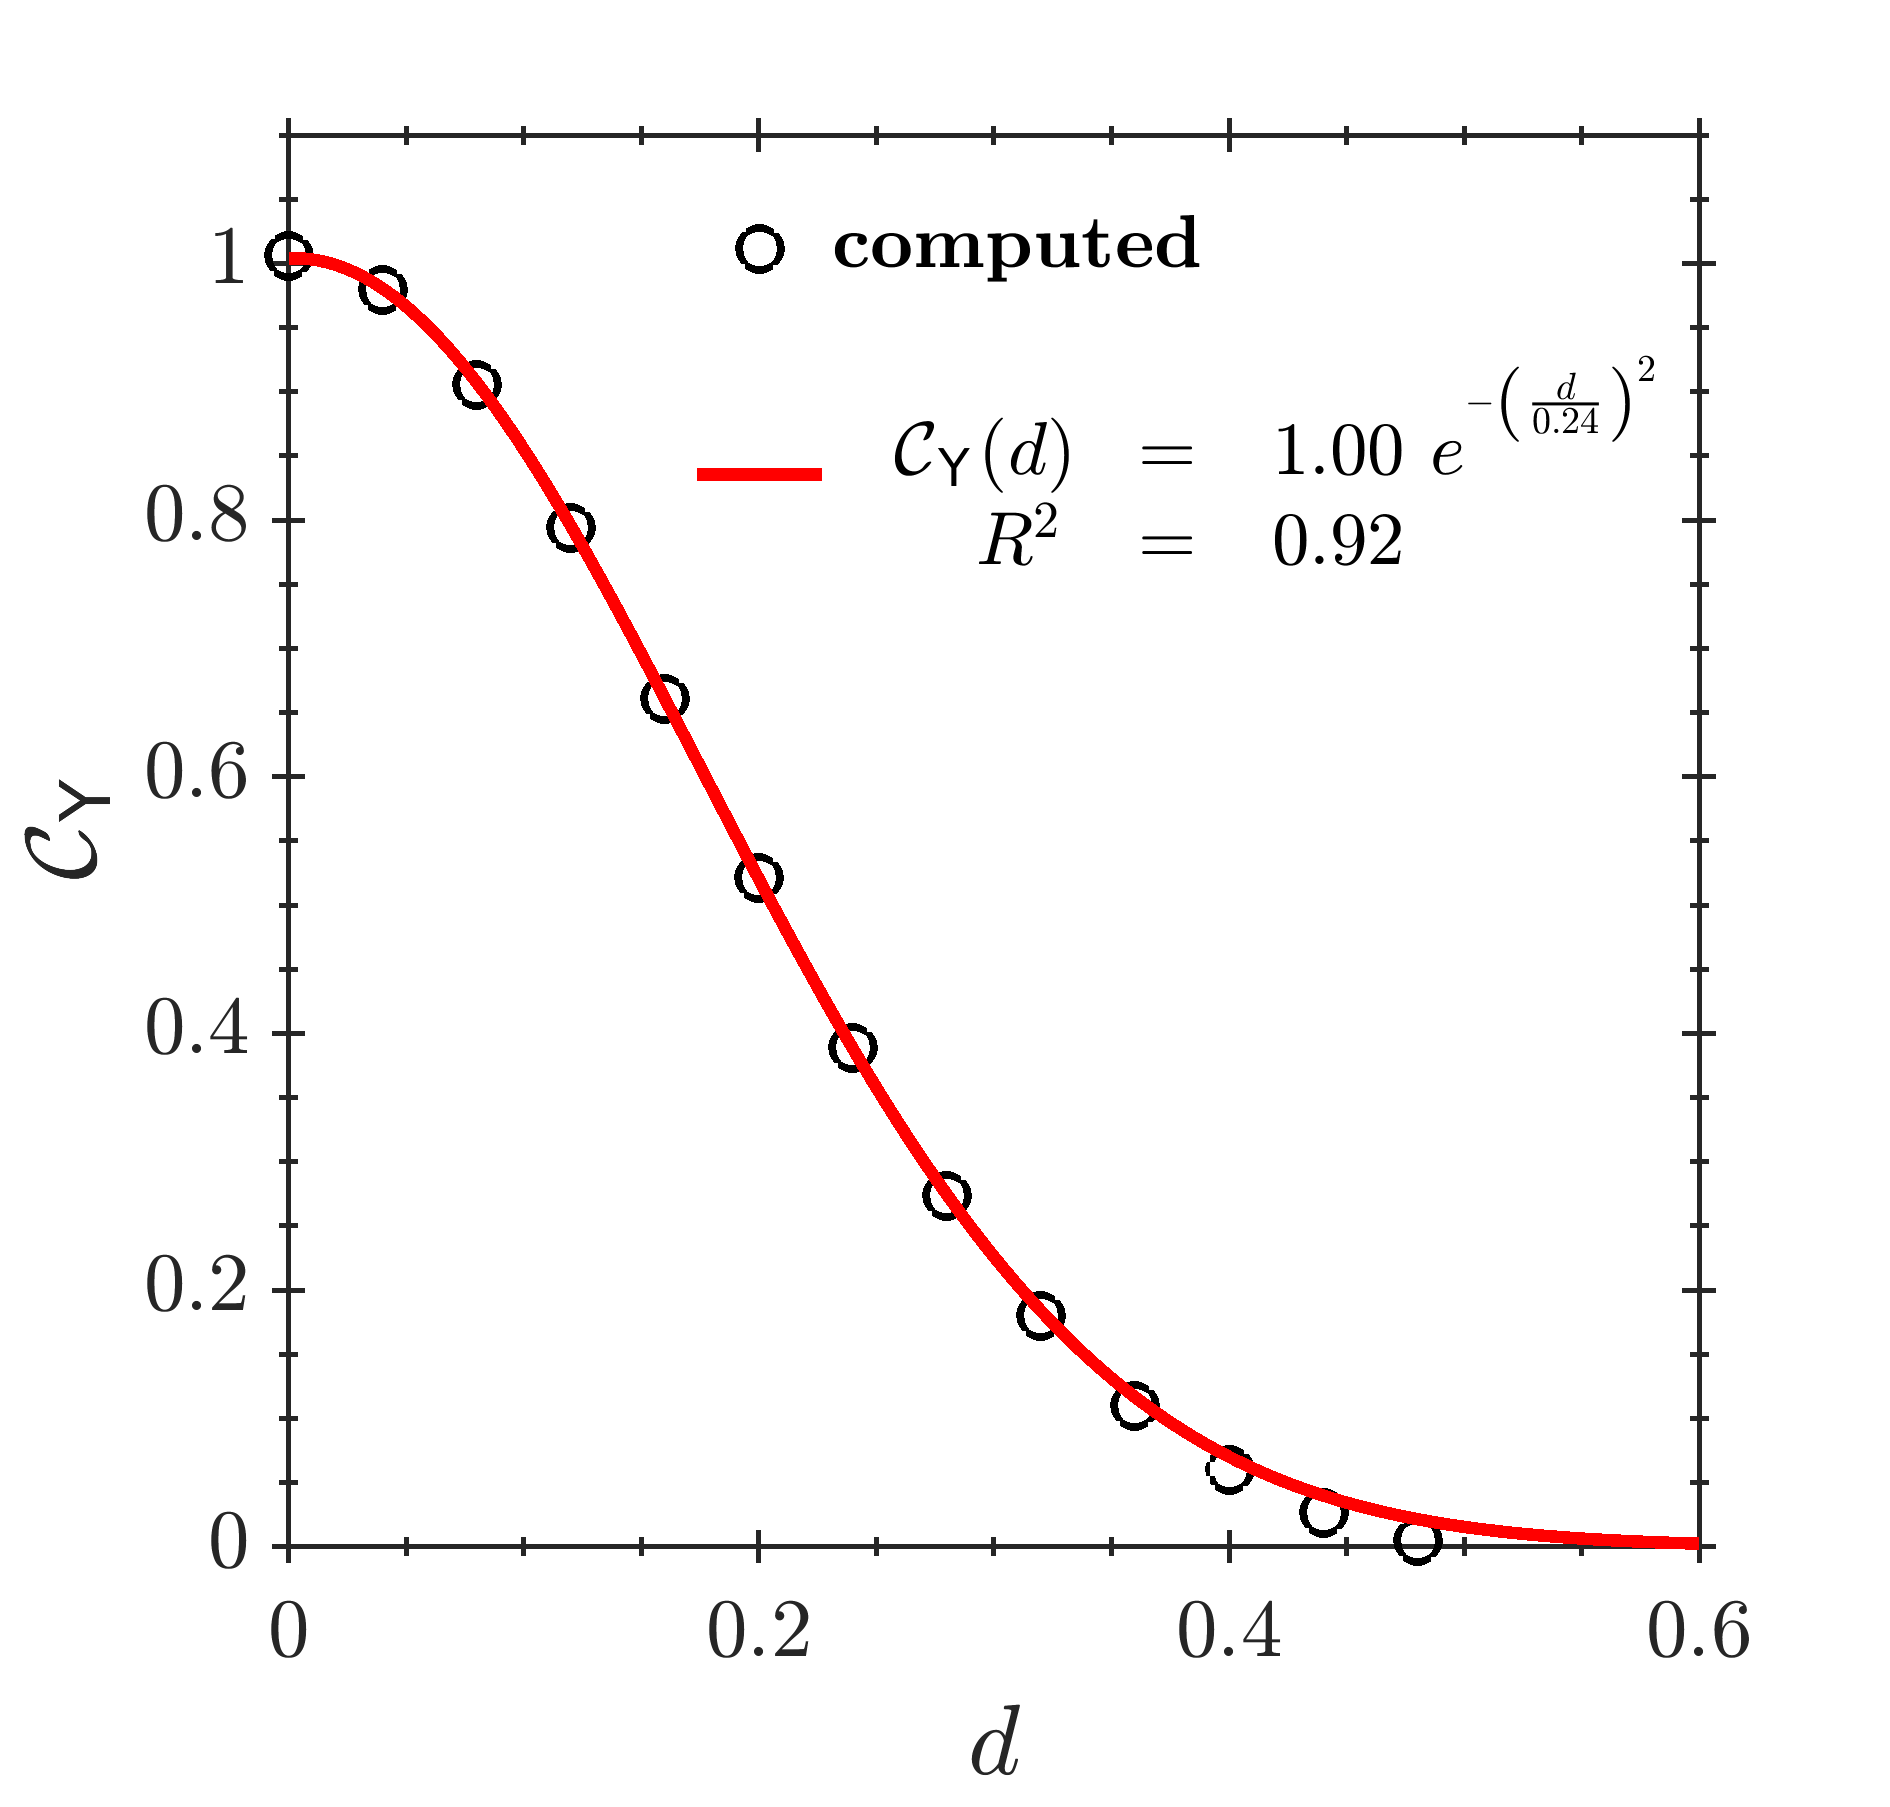
\includegraphics[scale = 0.325]{./figuras/e_gsexp_cond_1x0_6x0_4_25x15x10_0-2x0-2x0-1_5000_Yx.png}}
 \subfigure[Direction $y$]{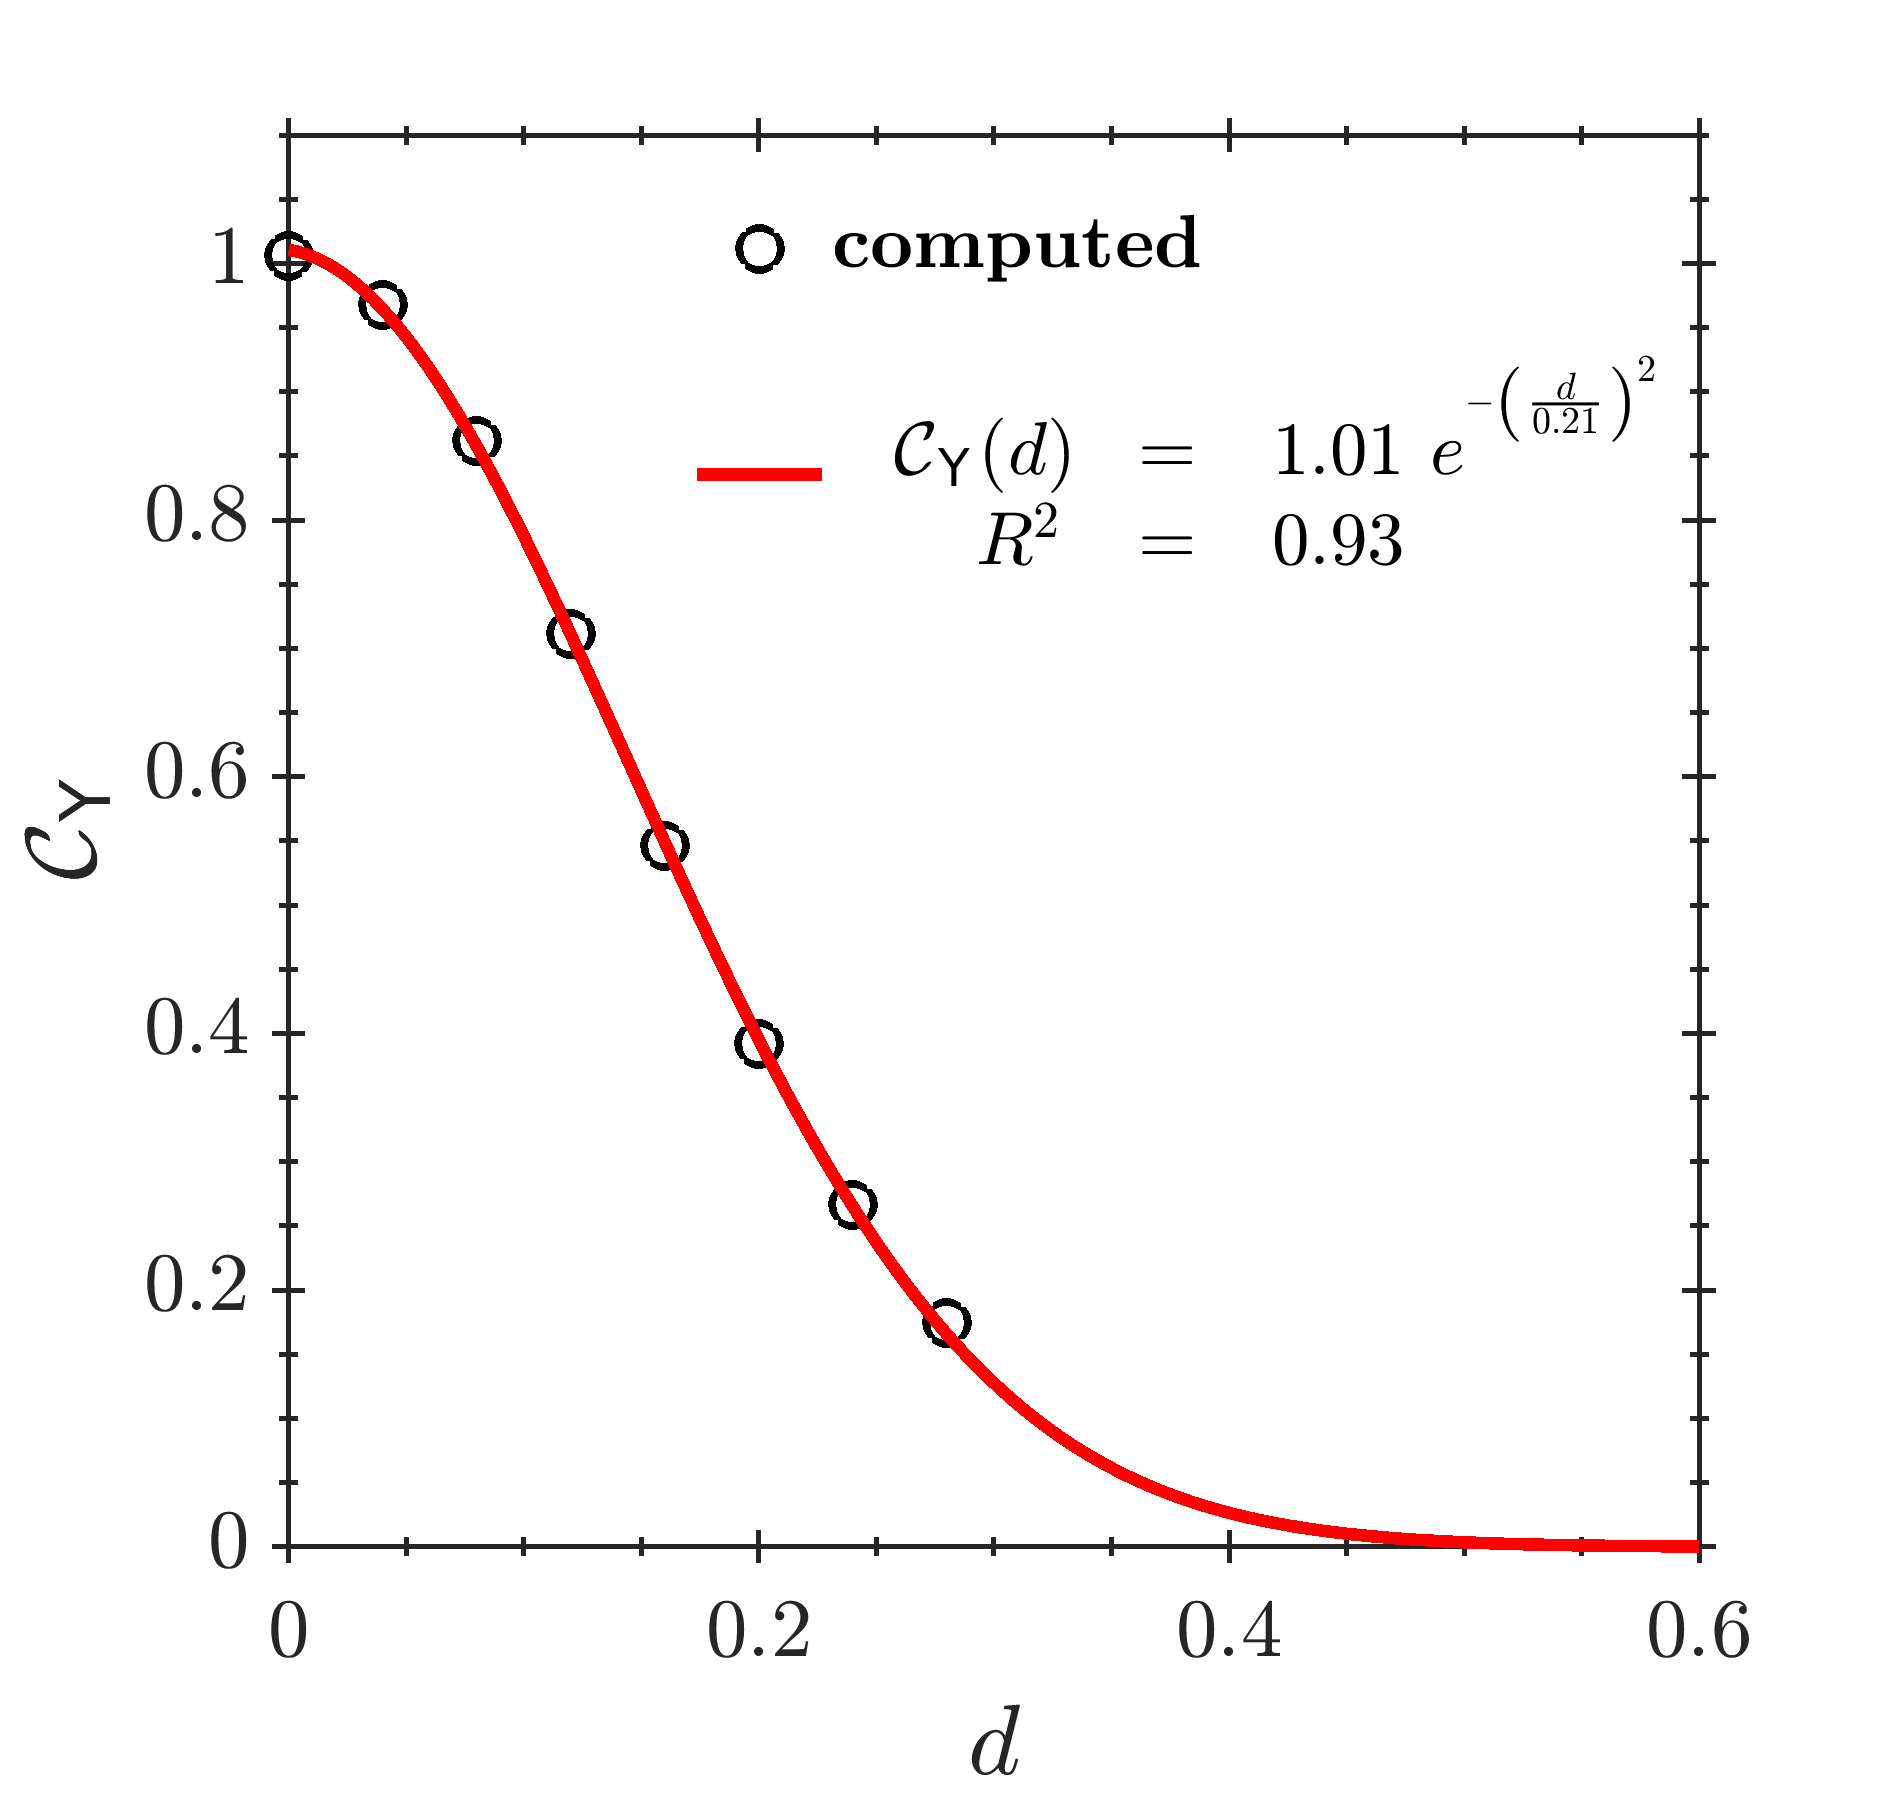
\includegraphics[scale = 0.325]{./figuras/e_gsexp_cond_1x0_6x0_4_25x15x10_0-2x0-2x0-1_5000_Yy.png}}
 \subfigure[Direction $z$]{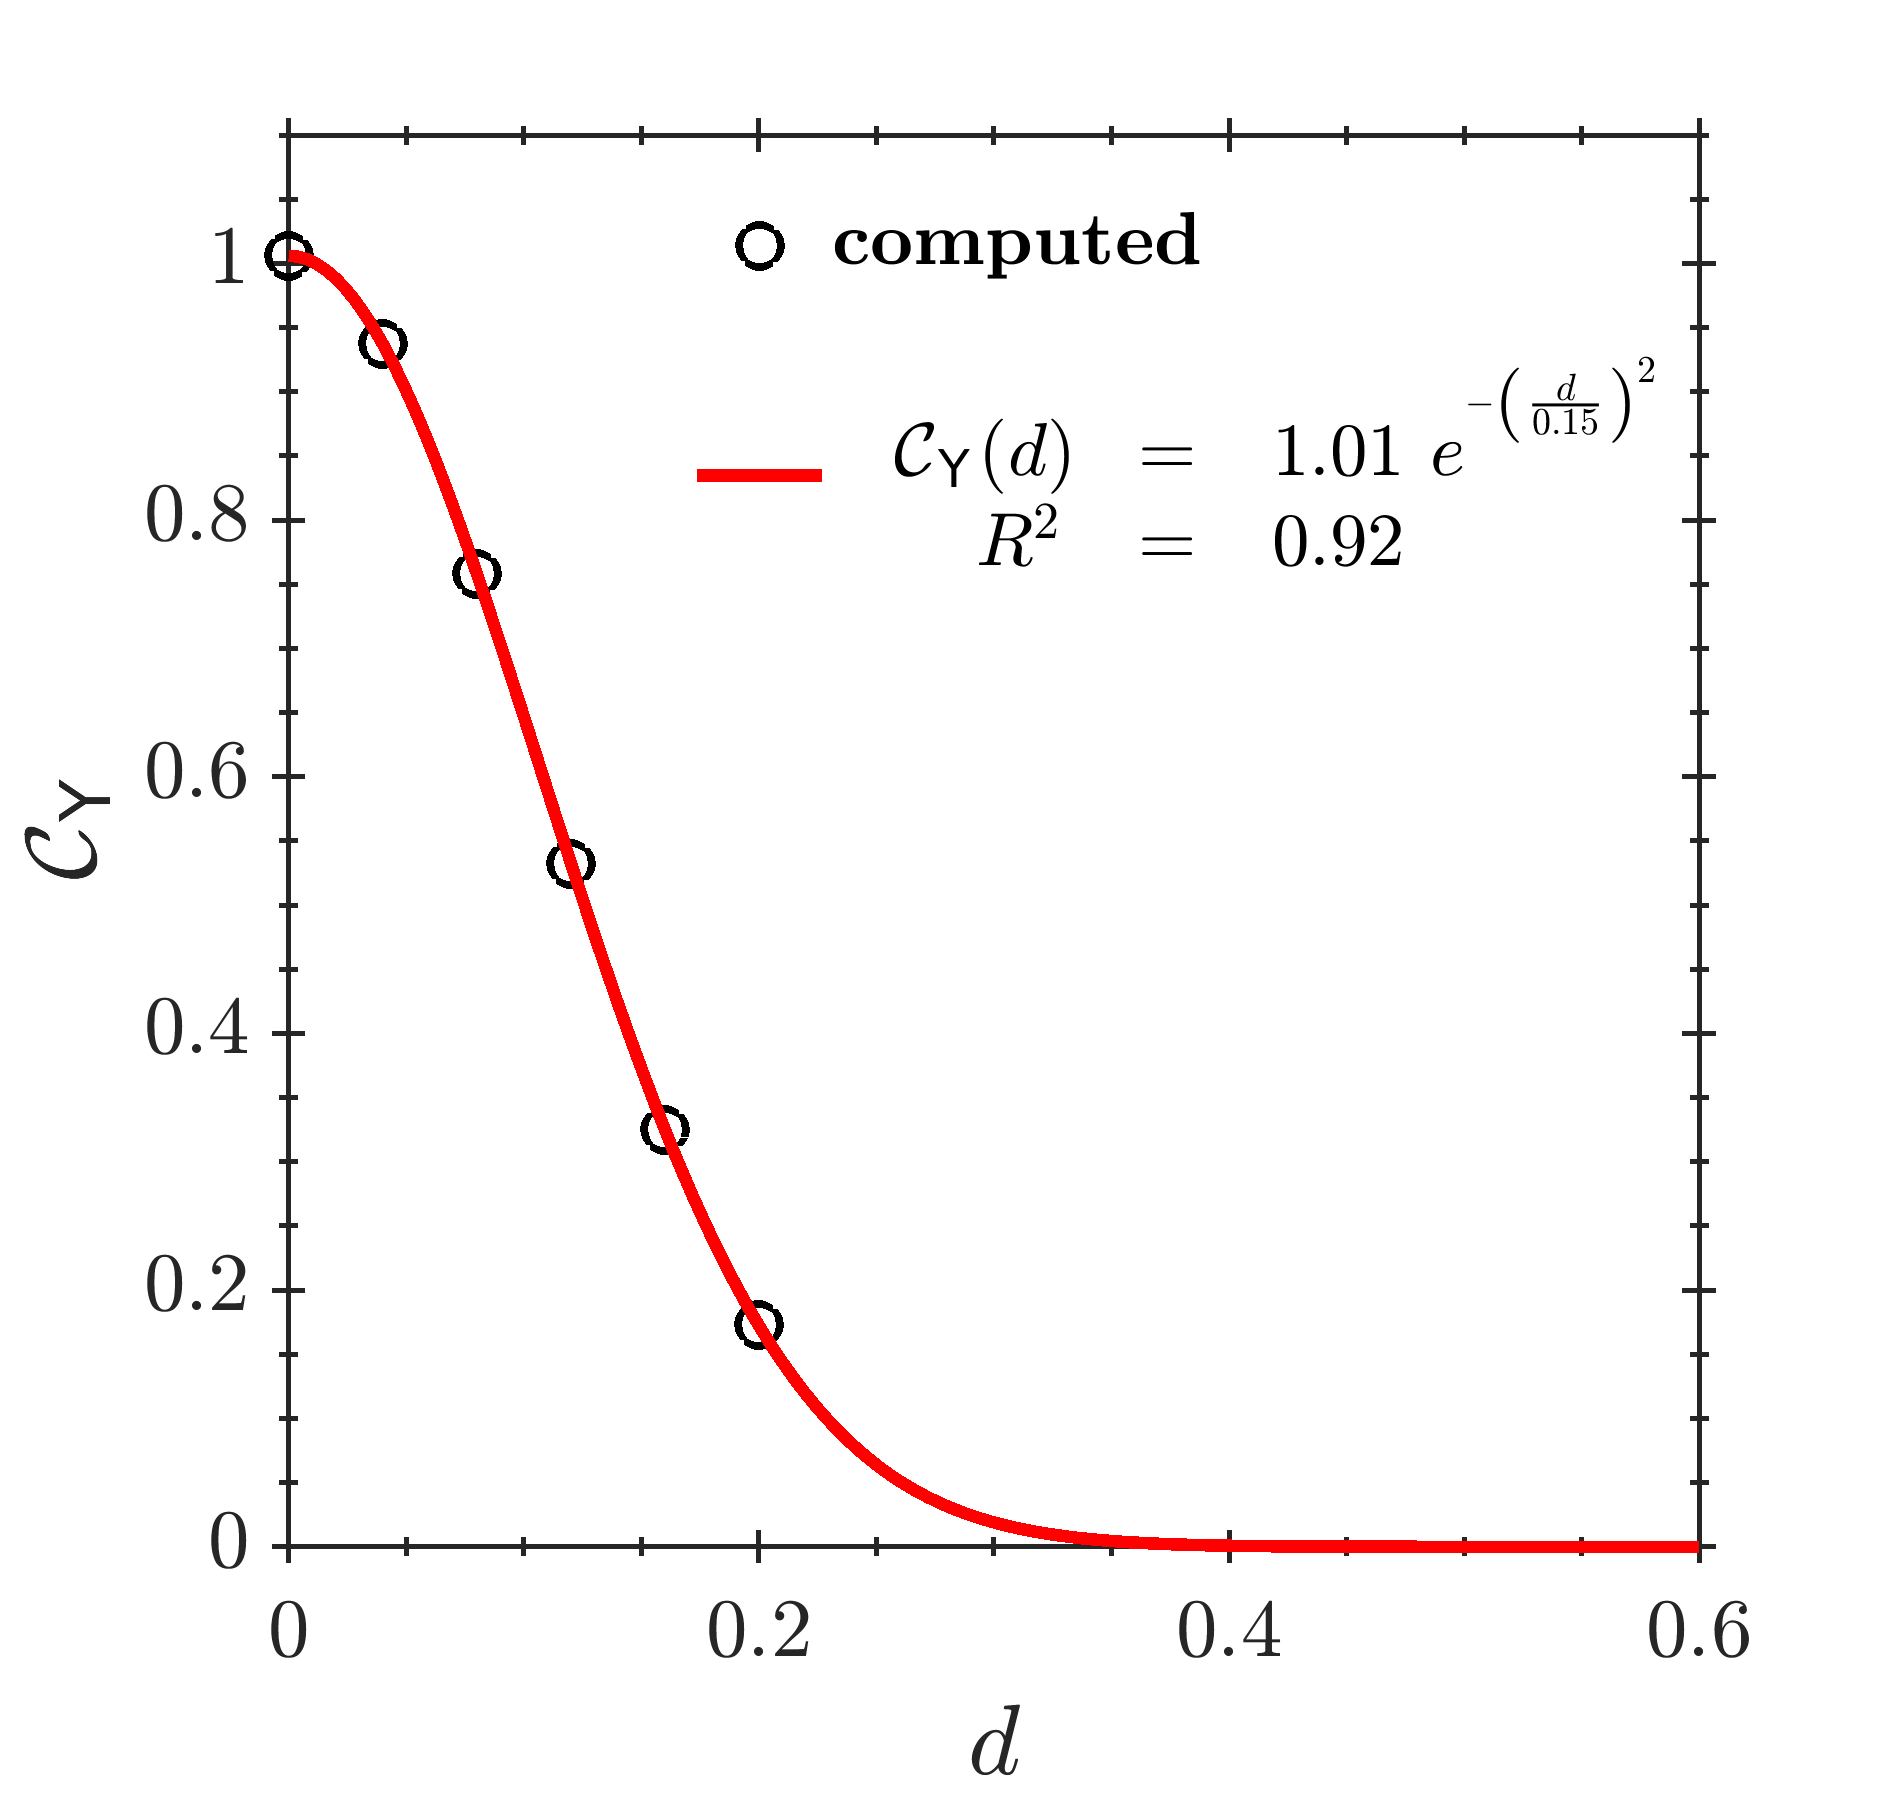
\includegraphics[scale = 0.325]{./figuras/e_gsexp_cond_1x0_6x0_4_25x15x10_0-2x0-2x0-1_5000_Yz.png}}
 \caption{Covariance as function of the lag distance $d=\lVert \vx - \vy \rVert$, computed with an ensamble of 2000 unconditioned fields.}
 \label{fig-uncondCov}
\end{figure}

%%%%%%%%%%%%%%%%%%%%%%%%%%%%%%%%%%%%%%%%%%%%%%%%%%%%%%%%%%%%%%%%%%
%%%%%%%%%%%%%%%%%%%%%%%%%%%%%%%%%%%%%%%%%%%%%%%%%%%%%%%%%%%%%%%%%%
\section{Synthetic experiment}
%%%%%%%%%%%%%%%%%%%%%%%%%%%%%%%%%%%%%%%%%%%%%%%%%%%%%%%%%%%%%%%%%%

We consider three-dimensional fields with dimensions: $36.0 \times 36.0 \times 50.0$ [$mm~\times~mm~\times~mm$] and mesh $36 \times 36 \times 50$.
Two kind of two-point covariance functions are considered:

\begin{itemize}
 \item Exponentially decaying covariance
 \begin{equation}
 \covv{\Y} = \vari{\Y}\exp\left(-\dfrac{\norma{x_1 - y_1}}{\cc_{1}}-\dfrac{\norma{x_2 - y_2}}{\cc_{2}}-\dfrac{\norma{x_3 - y_3}}{\cc_{3}}  \right),
 \label{eq-expcov}
\end{equation}

 \item Squared exponentially decaying covariance
\begin{equation}
 \covv{\Y} = \vari{\Y}\exp\left(-\dfrac{\norma{x_1 - y_1}^2}{\cc_{1}^{2}}-\dfrac{\norma{x_2 - y_2}^2}{\cc_{2}^{2}}-\dfrac{\norma{x_3 - y_3}^2}{\cc_{3}^{2}}  \right),
 \label{eq-squarecov}
\end{equation}
\end{itemize}

\noindent with $\vari{\Y}$ denoting the variance and $\cc_{i}>0,\ i=1,2,3$ the correlation length in each cartesian direction.
The correlation lengths used  in this study are: $\ell_{1}=\ell_{2}=\ell_{3}=3.0mm$.

Samples of the fields generated with \kl\ expansion are displayed in \figsto{fig-field_exp}{fig-field_sexp}

\begin{figure}[H]
 \centering
 \subfigure[Exponential]{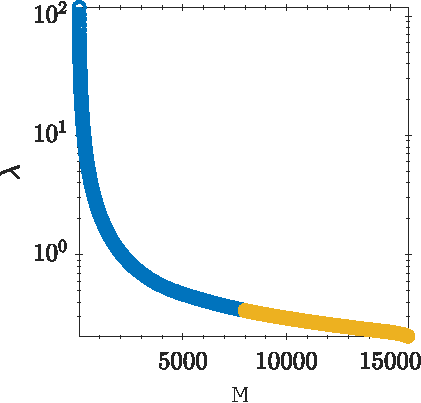
\includegraphics[scale=0.5]{./figuras/exp_autoval_36x36x50_3x3x3_8000.png}}
 \subfigure[Square exponential]{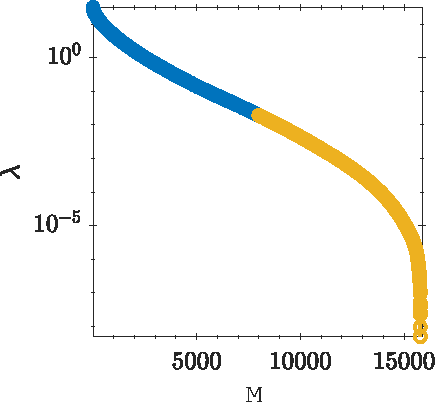
\includegraphics[scale=0.5]{./figuras/sexp_autoval_36x36x50_3x3x3_8000.png}}
 \caption{Eigenvalues of the covariance (\eq{kl}) as function of the number of terms in descending order.}
 \label{eigenval}
\end{figure}

%%%%%%%%%%%%%%%%%%%%%%%%%%%%%%%%%%%%%%%%%%%%%%%%%%%%%%%%%%%%%%%%%%
\begin{figure}[H]
 \centering
 \subfigure[]{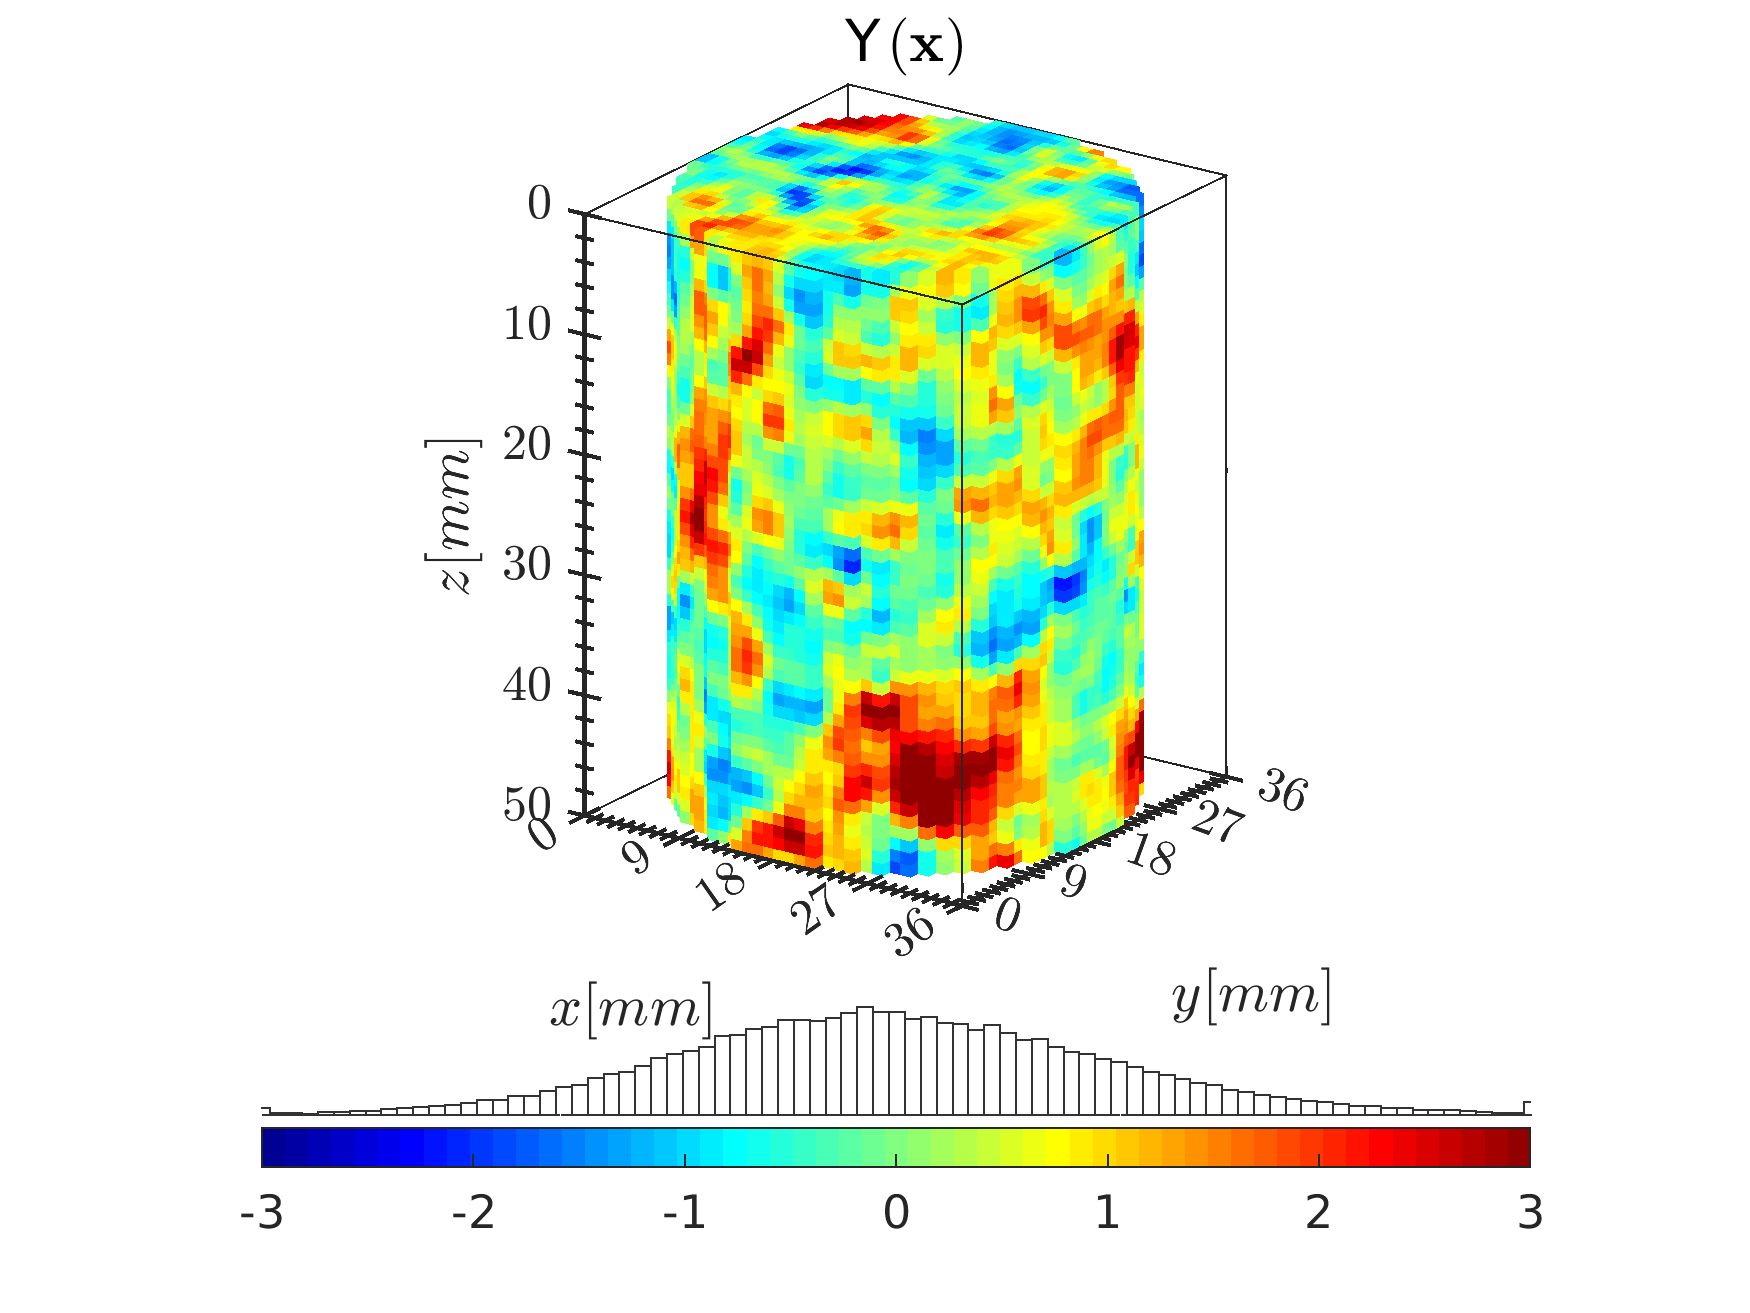
\includegraphics[scale=0.525]{./figuras/Y_TUBexpUNCOND_0.png}}
 \subfigure[]{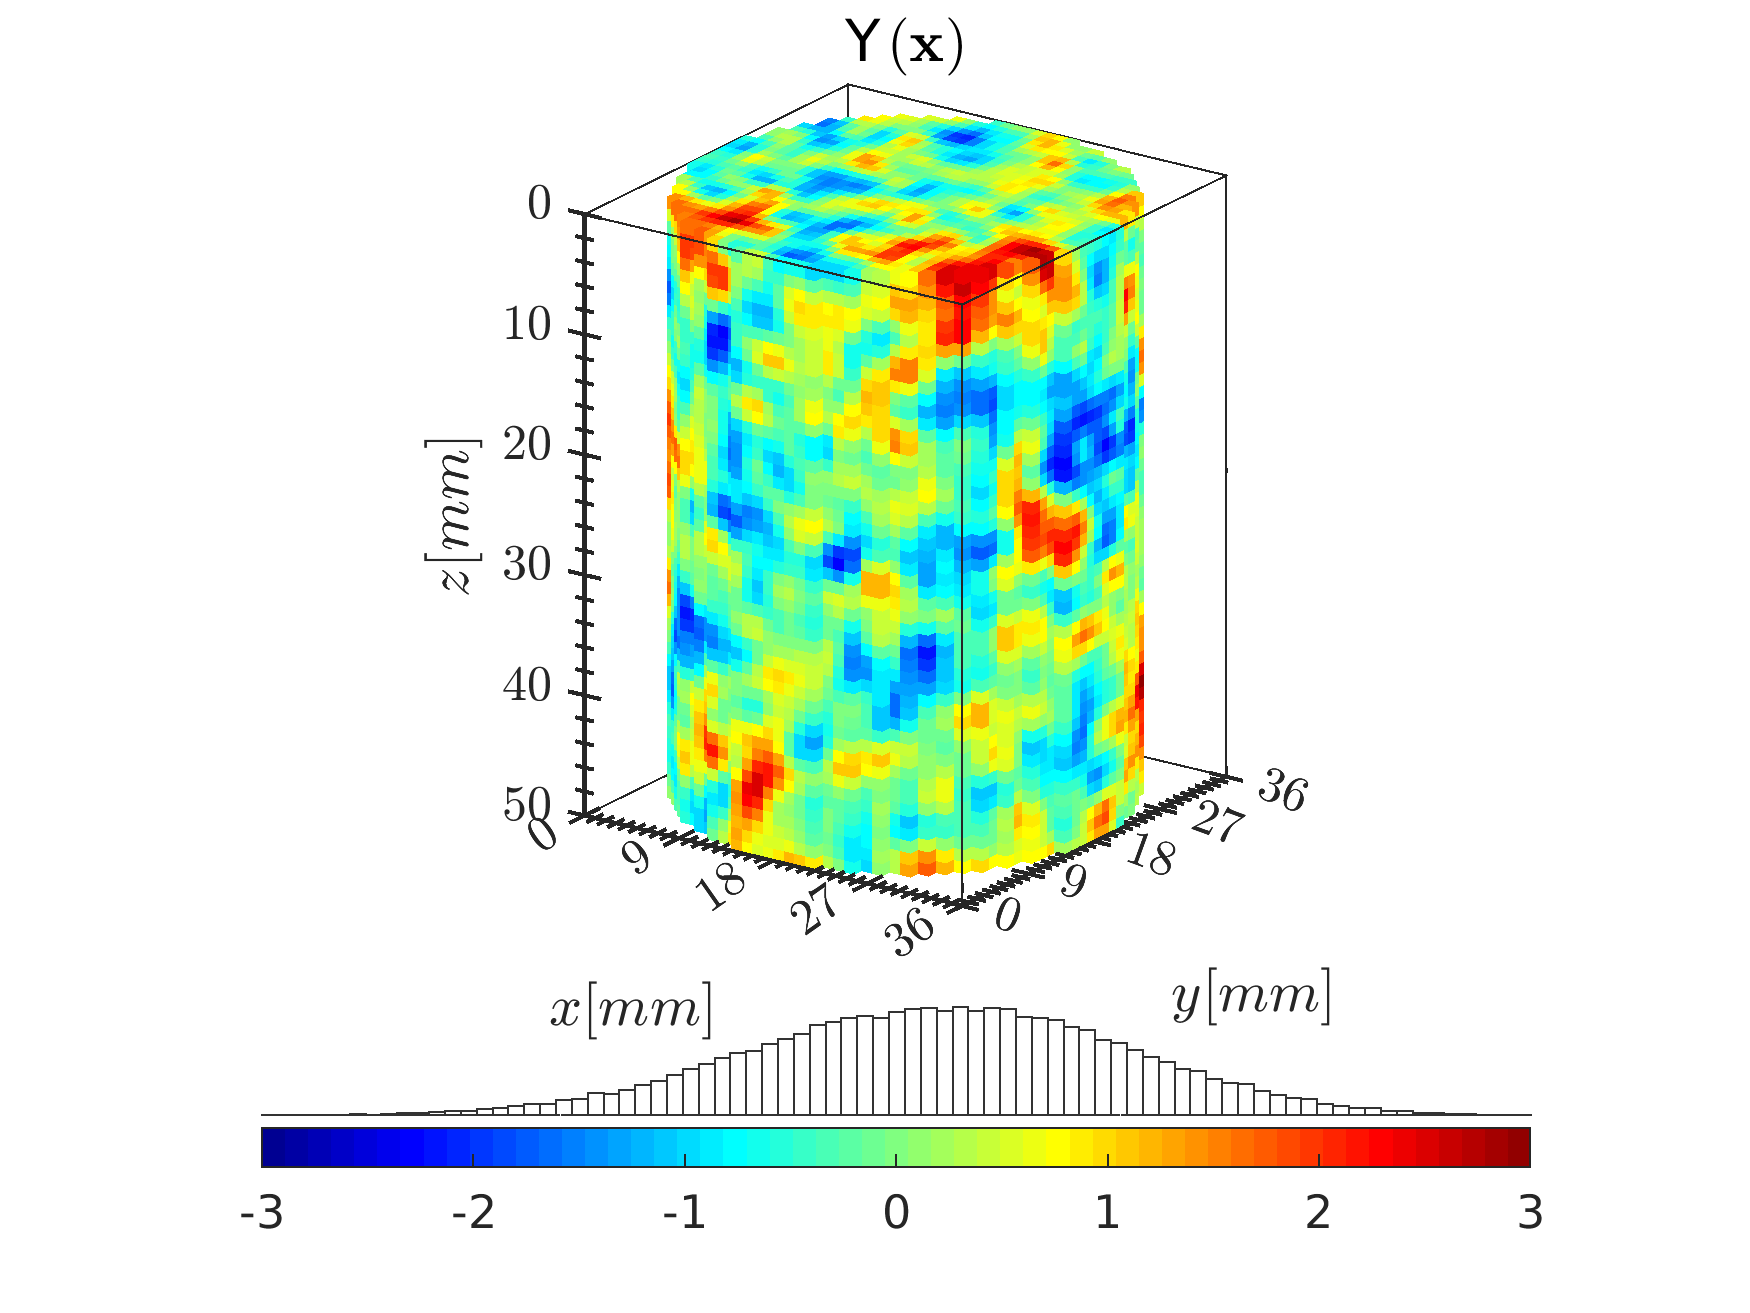
\includegraphics[scale=0.525]{./figuras/Y_TUBexpUNCOND_1.png}}
 \subfigure[]{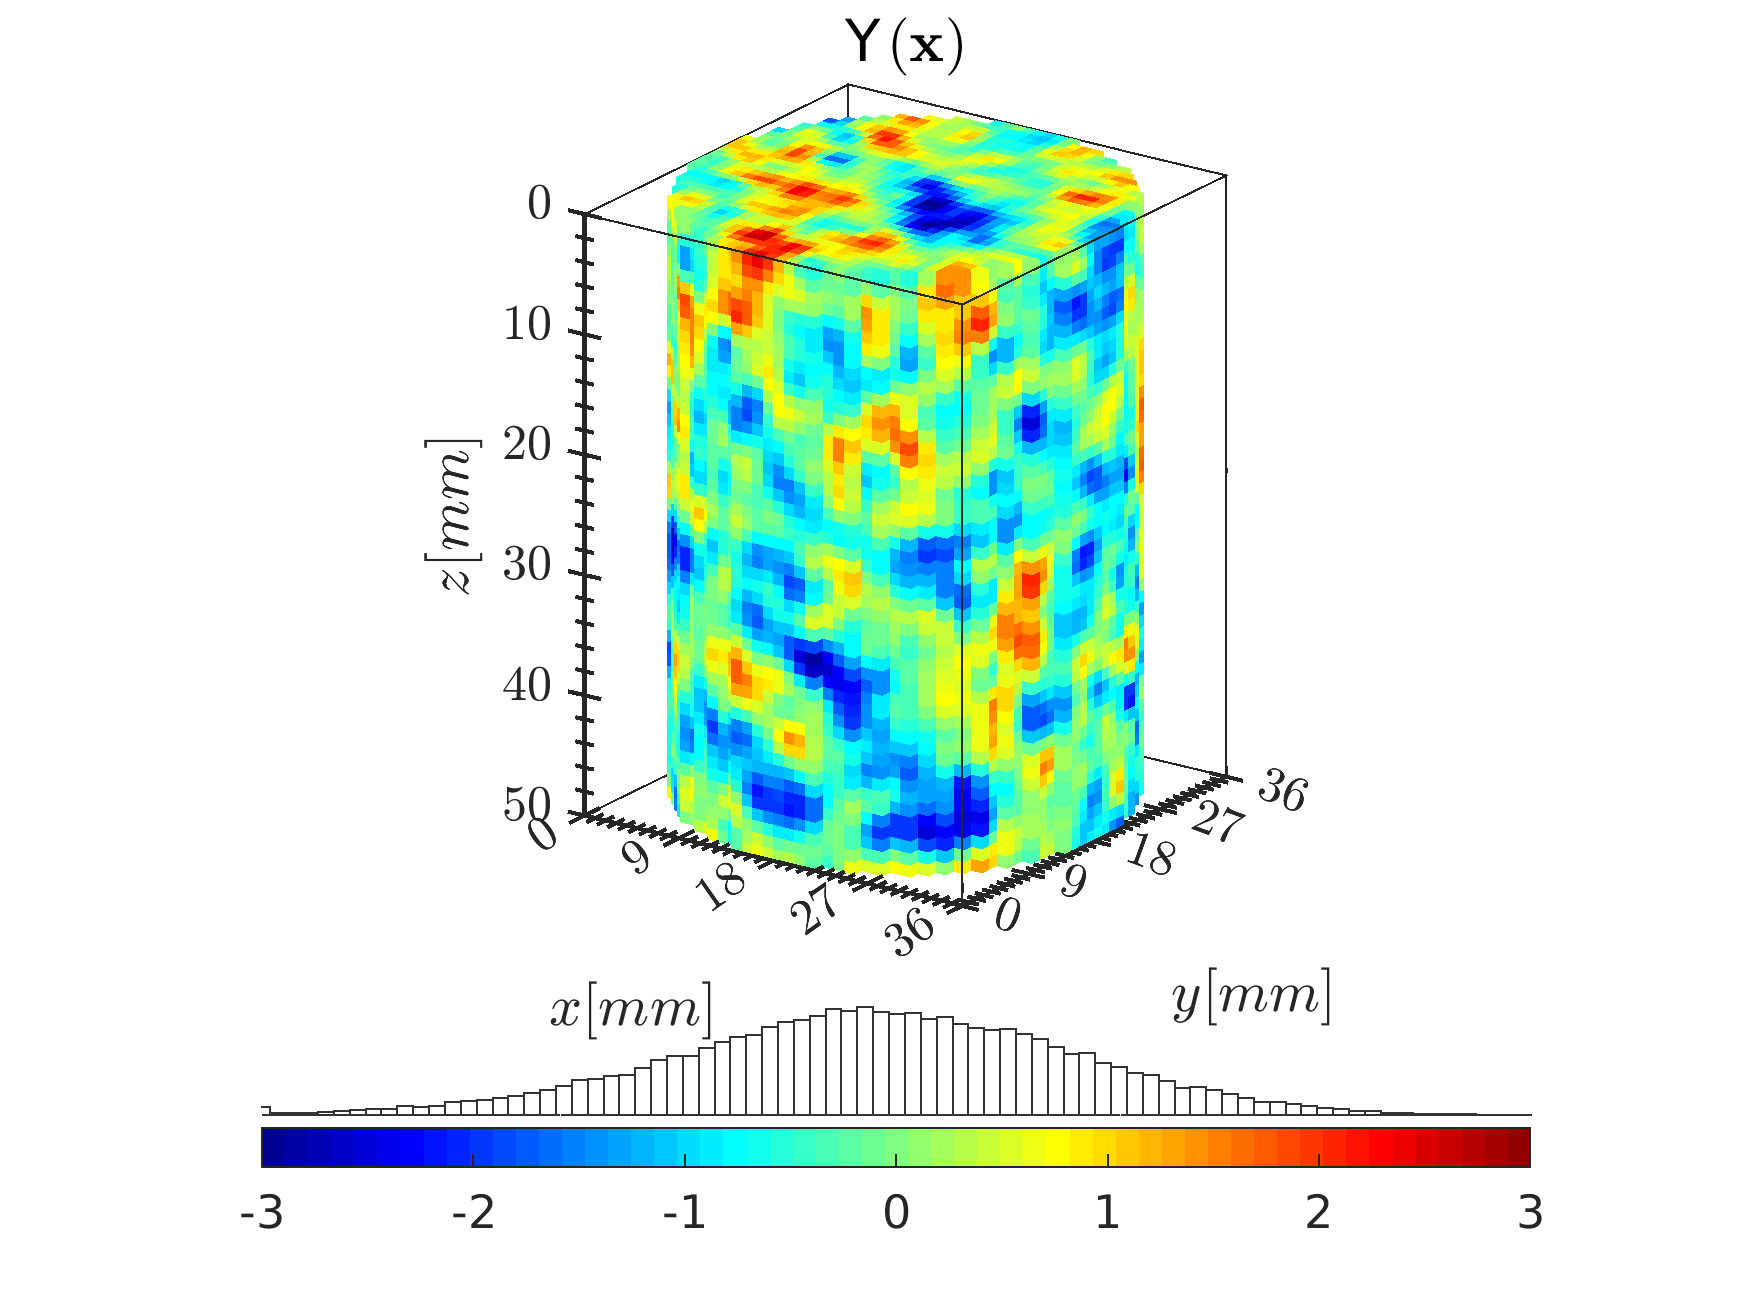
\includegraphics[scale=0.525]{./figuras/Y_TUBexpUNCOND_2.png}}
 \subfigure[]{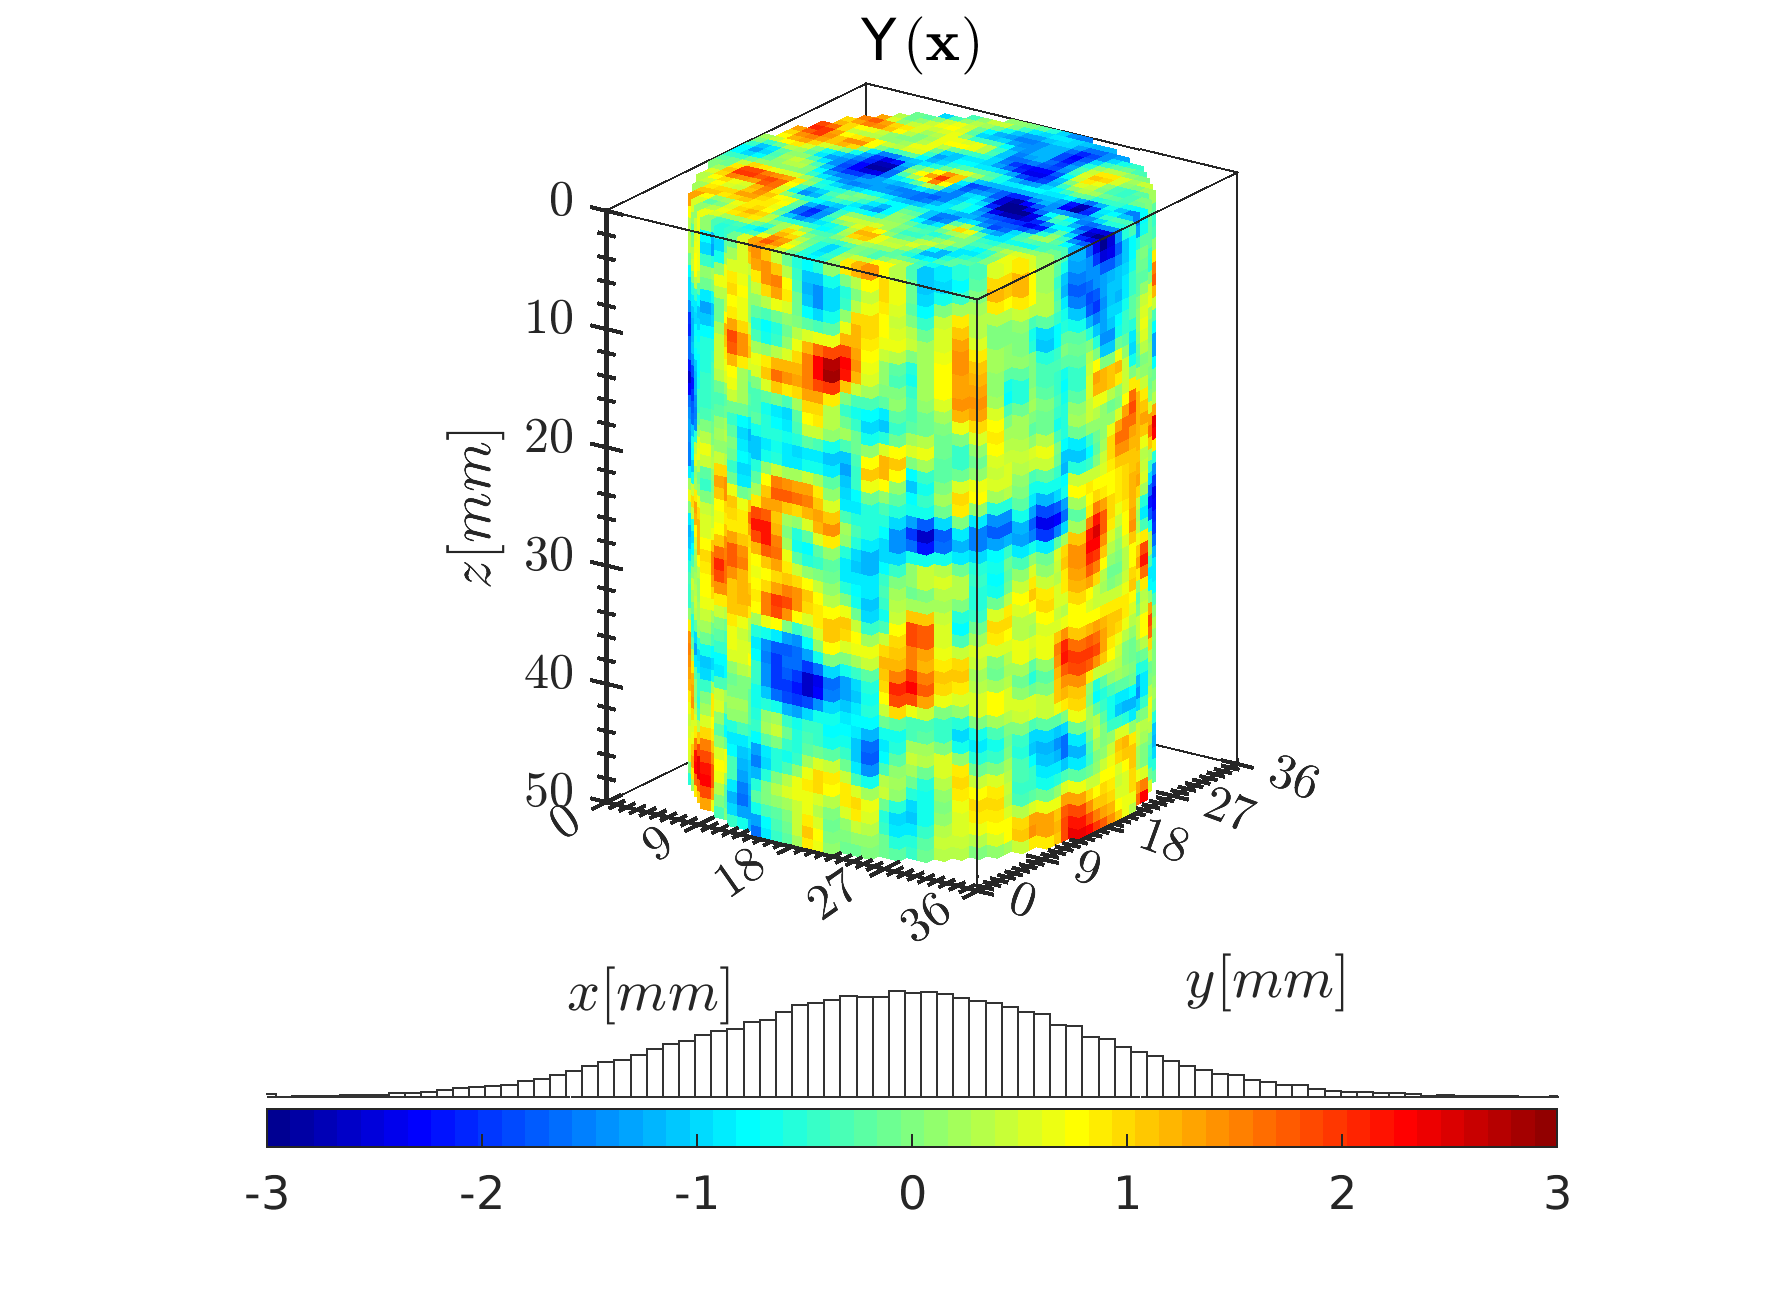
\includegraphics[scale=0.525]{./figuras/Y_TUBexpUNCOND_3.png}}
 \caption{Samples of random fields with exponentially decay covariance.}
 \label{fig-field_exp}
\end{figure}

%%%%%%%%%%%%%%%%%%%%%%%%%%%%%%%%%%%%%%%%%%%%%%%%%%%%%%%%%%%%%%%%%%
\begin{figure}[H]
 \centering
 \subfigure[]{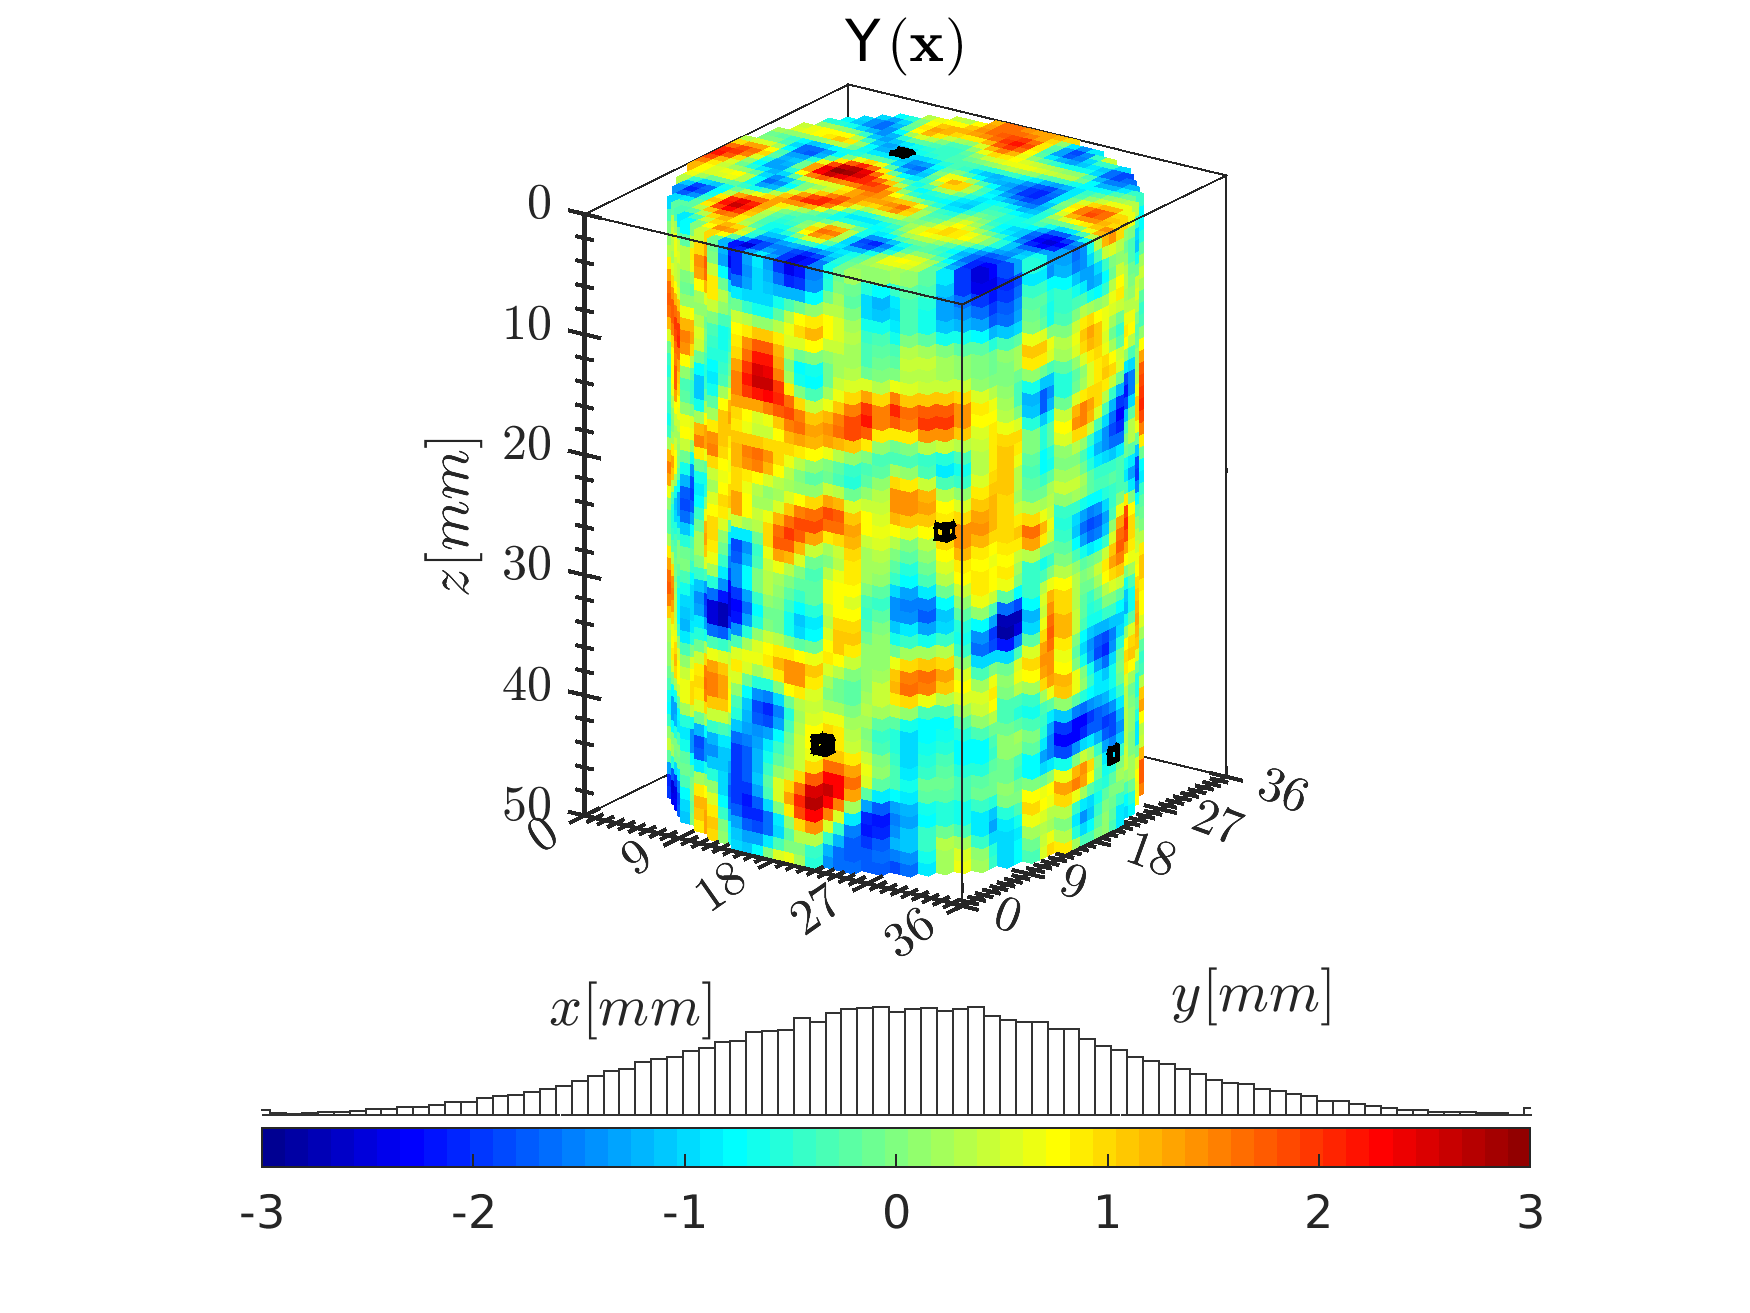
\includegraphics[scale=0.525]{./figuras/Y_TUBsexpCOND_0.png}}
 \subfigure[]{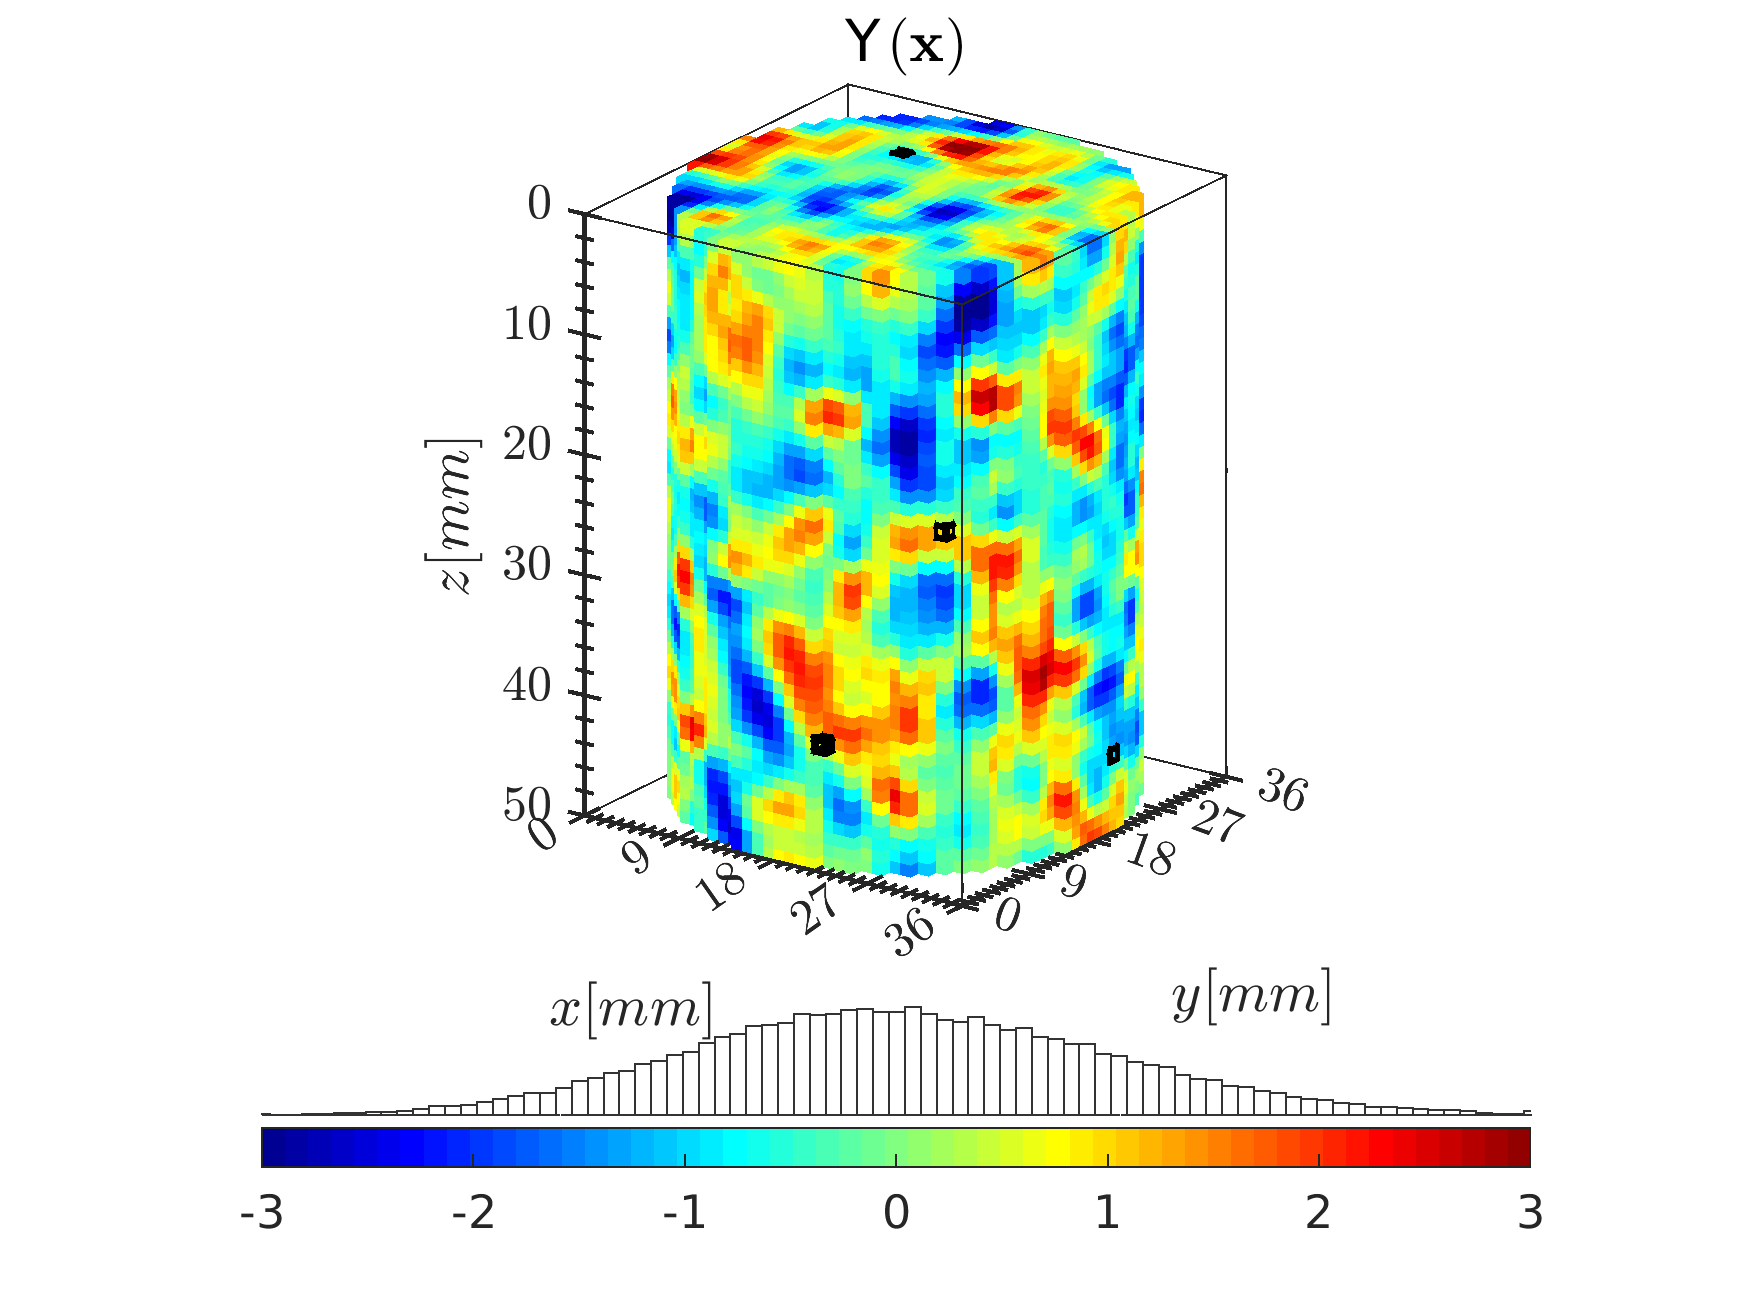
\includegraphics[scale=0.525]{./figuras/Y_TUBsexpCOND_1.png}}
 \subfigure[]{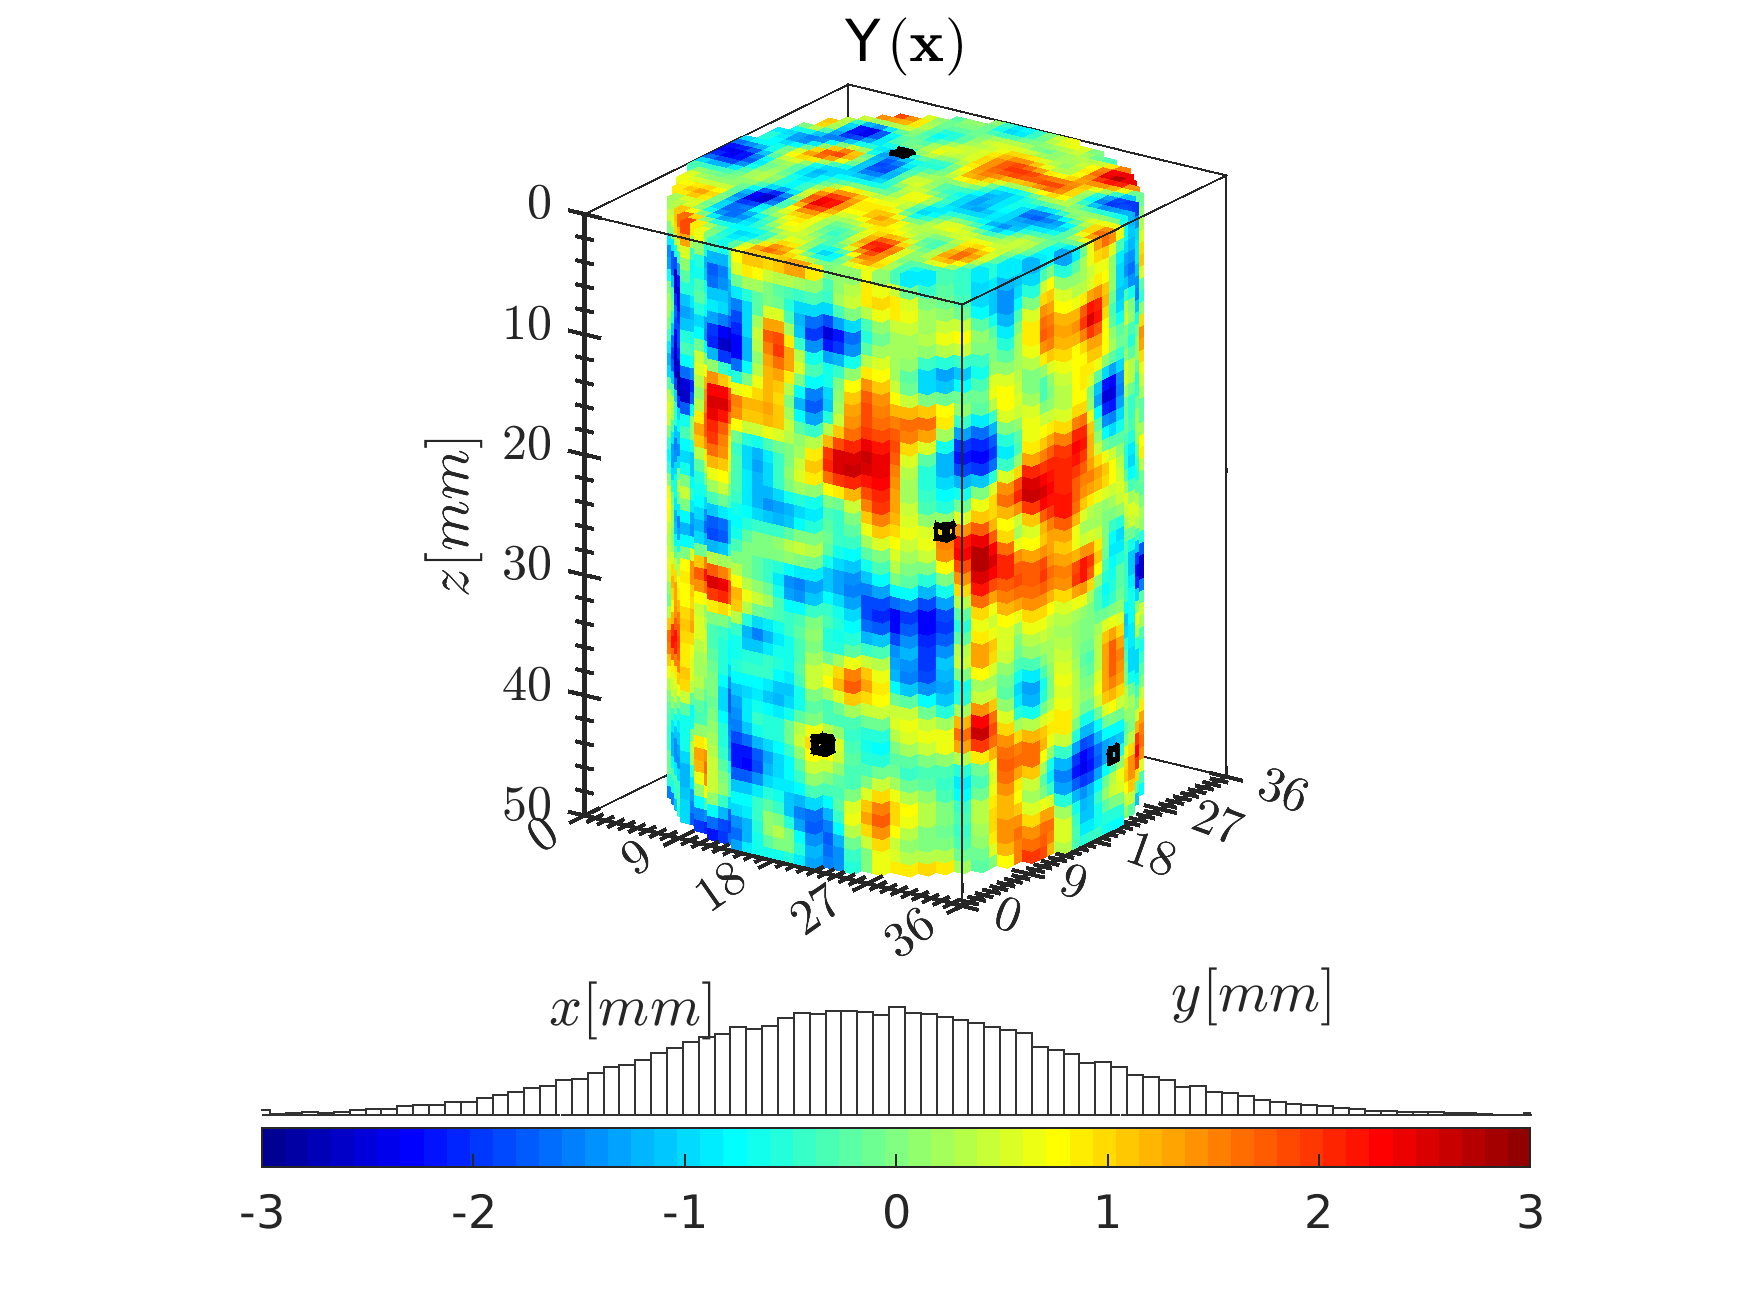
\includegraphics[scale=0.525]{./figuras/Y_TUBsexpCOND_2.png}}
 \subfigure[]{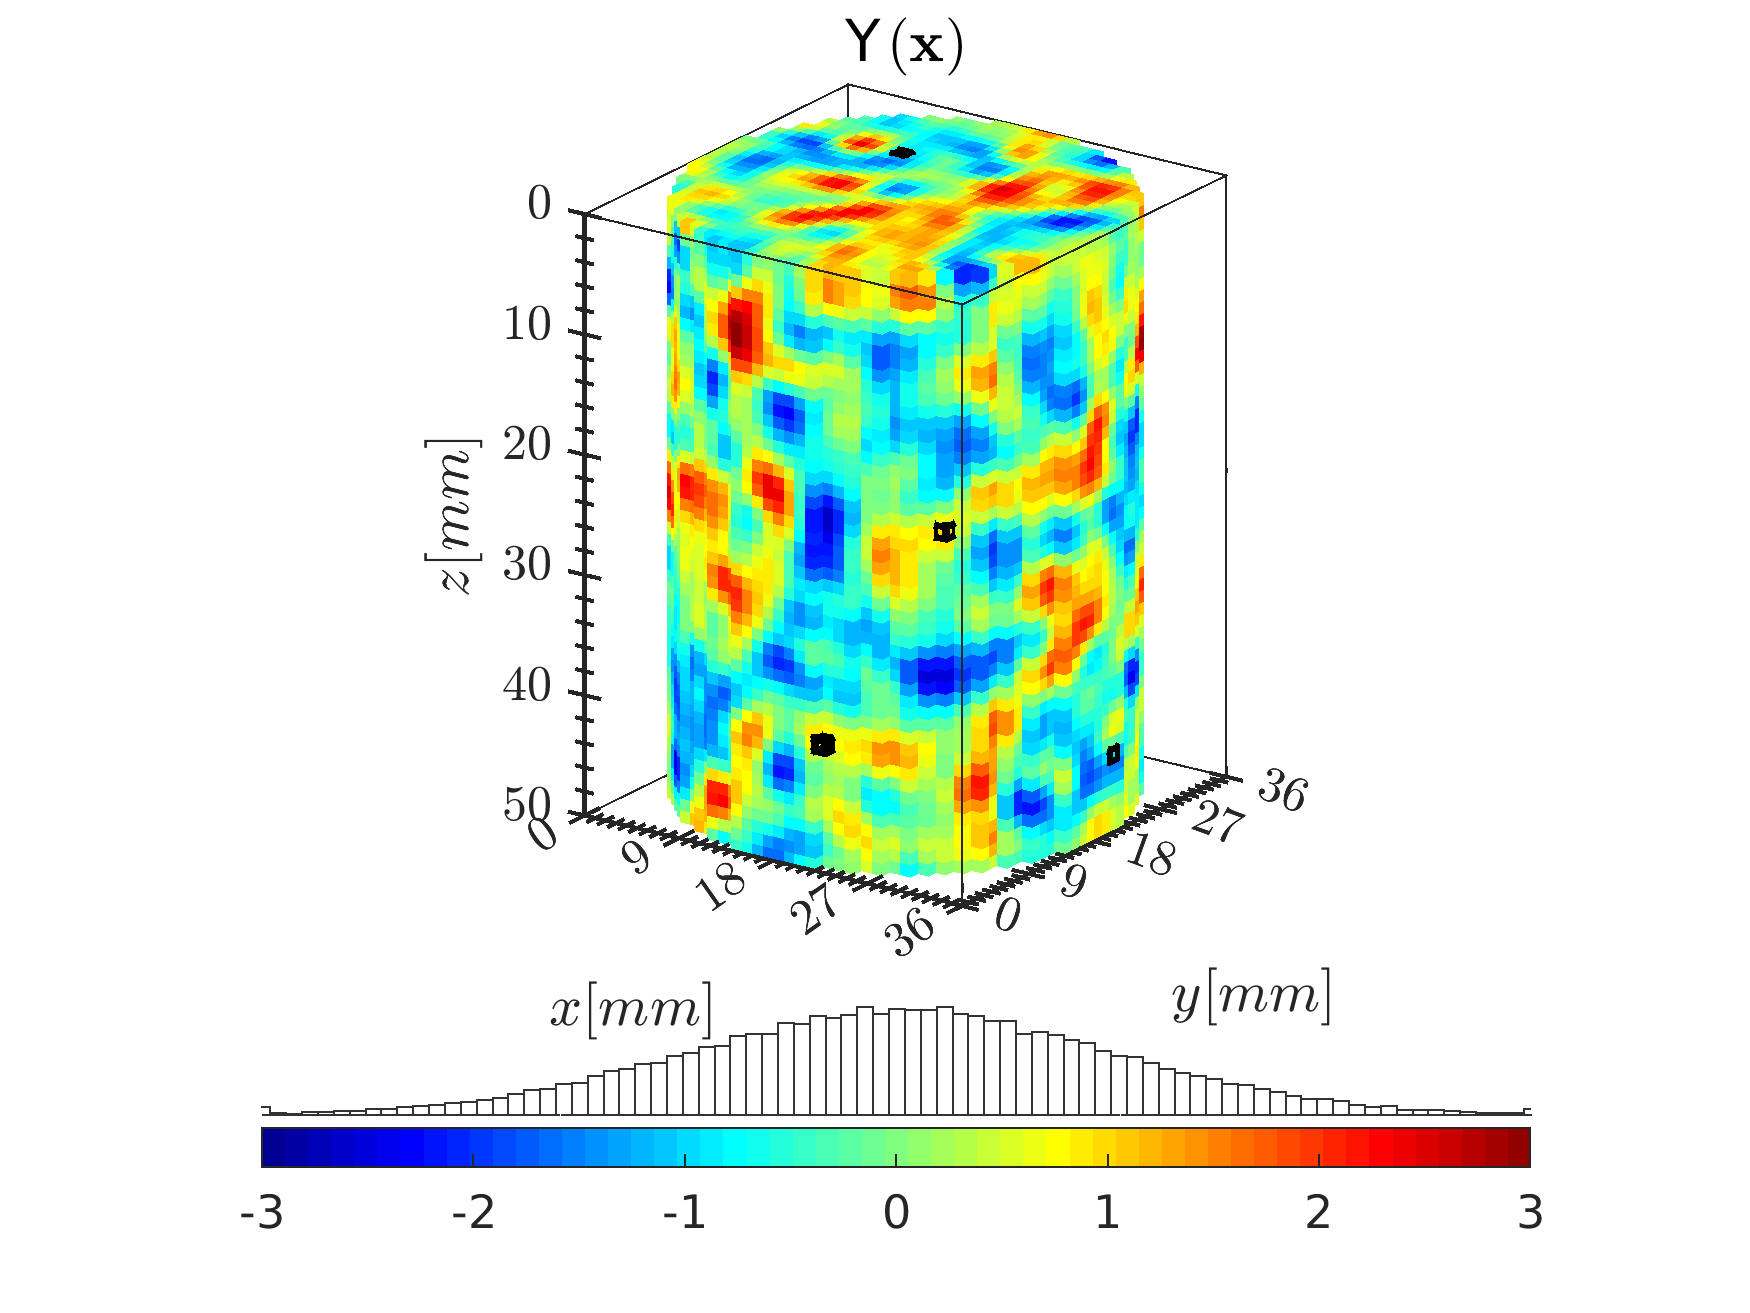
\includegraphics[scale=0.525]{./figuras/Y_TUBsexpCOND_3.png}}
 \caption{Samples of random fields with exponentially decay covariance.}
 \label{fig-field_sexp}
\end{figure}

%%%%%%%%%%%%%%%%%%%%%%%%%%%%%%%%%%%%%%%%%%%%%%%%%%%%%%%%%%%%%%%%%%
%%%%%%%%%%%%%%%%%%%%%%%%%%%%%%%%%%%%%%%%%%%%%%%%%%%%%%%%%%%%%%%%%%
%%%%%%%%%%%%%%%%%%%%%%%%%%%%%%%%%%%%%%%%%%%%%%%%%%%%%%%%%%%%%%%%%%
%%%%%%%%%%%%%%%%%%%%%%%%%%%%%%%%%%%%%%%%%%%%%%%%%%%%%%%%%%%%%%%%%%
%%%%%%%%%%%%%%%%%%%%%%%%%%%%%%%%%%%%%%%%%%%%%%%%%%%%%%%%%%%%%%%%%%
%%%%%%%%%%%%%%%%%%%%%%%%%%%%%%%%%%%%%%%%%%%%%%%%%%%%%%%%%%%%%%%%%%


% \begin{figure}[H]
%  \centering
%  \subfigure[Direction $x$]{\includegraphics[scale=0.325]{./figuras/e_gexp_40x40x40_20x20x20_10x8x6_2000_Yx.png}}
%  \subfigure[Direction $y$]{\includegraphics[scale=0.325]{./figuras/e_gexp_40x40x40_20x20x20_10x8x6_2000_Yy.png}}
%  \subfigure[Direction $z$]{\includegraphics[scale=0.325]{./figuras/e_gexp_40x40x40_20x20x20_10x8x6_2000_Yz.png}}
%  \subfigure[Direction $x$]{\includegraphics[scale=0.325]{./figuras/eIn_gexp_40x40x40_20x20x20_10x8x6_2000_Yx.png}}
%  \subfigure[Direction $y$]{\includegraphics[scale=0.325]{./figuras/eIn_gexp_40x40x40_20x20x20_10x8x6_2000_Yy.png}}
%  \subfigure[Direction $z$]{\includegraphics[scale=0.325]{./figuras/eIn_gexp_40x40x40_20x20x20_10x8x6_2000_Yz.png}}
%  \subfigure[Direction $x$]{\includegraphics[scale=0.325]{./figuras/eM_gexp_40x40x40_20x20x20_10x8x6_2000_Yx.png}}
%  \subfigure[Direction $y$]{\includegraphics[scale=0.325]{./figuras/eM_gexp_40x40x40_20x20x20_10x8x6_2000_Yy.png}}
%  \subfigure[Direction $z$]{\includegraphics[scale=0.325]{./figuras/eM_gexp_40x40x40_20x20x20_10x8x6_2000_Yz.png}}
%  \caption{Computed covariance as function of the lag distance $r=\lVert \vx - \vy \rVert$.}
%  \label{figcovexp}
% \end{figure}
% 
% \begin{figure}[H]
%  \centering
%  \subfigure[Direction $x$]{\includegraphics[scale=0.325]{./figuras/e_gsexp_40x40x40_20x20x20_10x8x6_2000_Yx.png}}
%  \subfigure[Direction $y$]{\includegraphics[scale=0.325]{./figuras/e_gsexp_40x40x40_20x20x20_10x8x6_2000_Yy.png}}
%  \subfigure[Direction $z$]{\includegraphics[scale=0.325]{./figuras/e_gsexp_40x40x40_20x20x20_10x8x6_2000_Yz.png}}
%  \subfigure[Direction $x$]{\includegraphics[scale=0.325]{./figuras/eIn_gsexp_40x40x40_20x20x20_10x8x6_2000_Yx.png}}
%  \subfigure[Direction $y$]{\includegraphics[scale=0.325]{./figuras/eIn_gsexp_40x40x40_20x20x20_10x8x6_2000_Yy.png}}
%  \subfigure[Direction $z$]{\includegraphics[scale=0.325]{./figuras/eIn_gsexp_40x40x40_20x20x20_10x8x6_2000_Yz.png}}
%  \caption{Computed covariance as function of the lag distance $r=\lVert \vx - \vy \rVert$.}
%  \label{figcovexpf}
% \end{figure}
% 
% 
% \begin{figure}[H]
%  \centering
%  \subfigure[]{\includegraphics[scale=0.3]{./figuras/fields3D_cond_0001.png}}
%  \subfigure[]{\includegraphics[scale=0.3]{./figuras/fields3D_cond_0002.png}}\\
%  \subfigure[]{\includegraphics[scale=0.3]{./figuras/fields3D_cond_0003.png}}
%  \subfigure[]{\includegraphics[scale=0.3]{./figuras/fields3D_cond_0000.png}}
% \end{figure}



